% Coordinated prefetch throttling and LLC partitioning -- ACA course project report
% Build: latexmk -pdf main.tex   (or pdflatex main; bibtex main; pdflatex main; pdflatex main)
% Uses IEEEtran when available (e.g. Overleaf); falls back to a two-column article otherwise.
\IfFileExists{IEEEtran.cls}{\documentclass[conference]{IEEEtran}}{\documentclass[10pt,twocolumn]{article}}

\makeatletter
\@ifclassloaded{IEEEtran}{}{%
  \usepackage[margin=0.75in,columnsep=0.25in]{geometry}%
}
\makeatother

\usepackage[T1]{fontenc}
\usepackage{lmodern}
\usepackage{microtype}
\usepackage{amsmath,amssymb}
\usepackage{graphicx}
\usepackage{booktabs}
\usepackage{multirow}
\usepackage{xcolor}
\usepackage{tikz}
\usetikzlibrary{arrows.meta,positioning,fit,calc,shapes.geometric,backgrounds}
\usepackage[ruled,vlined,linesnumbered]{algorithm2e}
\usepackage[hidelinks]{hyperref}
\usepackage[capitalise,noabbrev]{cleveref}

\graphicspath{{figures/}}
% let LaTeX place floats near their text instead of deferring them to the end
\renewcommand{\topfraction}{0.9}\renewcommand{\dbltopfraction}{0.9}
\renewcommand{\bottomfraction}{0.6}\renewcommand{\textfraction}{0.07}
\renewcommand{\floatpagefraction}{0.6}\renewcommand{\dblfloatpagefraction}{0.6}
\setcounter{topnumber}{4}\setcounter{dbltopnumber}{3}\setcounter{totalnumber}{6}
\makeatletter   % float-only pages: stack floats at the top instead of centring them with large gaps
\setlength{\@fptop}{0pt}\setlength{\@fpsep}{14pt plus 2pt}\setlength{\@fpbot}{0pt plus 1fil}
\setlength{\@dblfptop}{0pt}\setlength{\@dblfpsep}{14pt plus 2pt}\setlength{\@dblfpbot}{0pt plus 1fil}
\makeatother
\newcommand{\pending}[1]{\textcolor{red}{[\textbf{Pending:} #1]}}
\newcommand{\vthree}{TSC}
\InputIfFileExists{tables/oracle_numbers}{}{}   % oracle numbers quoted in Section 3 (scripts/make_figures.py)

\title{Throughput-Safe Coordination of Prefetch Throttling and\\Shared-LLC Partitioning in Bandwidth-Constrained Multi-Cores}

\author{%
  \textit{ACA Course Project}\\
  \pending{author names and affiliation}
}

\date{}

\begin{document}
\maketitle

\begin{abstract}
Hardware prefetchers and shared last-level-cache (LLC) partitioning are designed and deployed independently, yet they
compete for the same two resources: LLC capacity and DRAM bandwidth.  Using ChampSim with two state-of-the-art
prefetchers (IPCP and Pythia) and Utility-based Cache Partitioning (UCP), we show that on 8 cores at 2.4\,GB/s per core, 36\% (IPCP) and 26\% (Pythia) of the cores run more than 2\% slower
than with neither mechanism, that UCP changes the allocation of few cores when prefetching is enabled, and that with
IPCP the cores that gain ways have inaccurate prefetchers.  A static oracle finds up to 38\% of headroom at 8 cores,
against \OrcIpMean\% (IPCP) and \OrcPyMean\% (Pythia) on average on 4 cores with ample bandwidth.  Prior-style
fairness-driven throttling keeps the cores that prefetching speeds up by at least 1.3$\times$ throttled about 90\% of
the time and loses up to 16\% on individual mixes.  We present TSC, a modular, epoch-based Throughput-Safe
Coordinator that (i)~applies each throttle step tentatively and keeps it only if the IPC measured in the following epochs shows at most
0.5\% throughput loss and at most 1\% loss for the throttled core, cutting the \emph{farthest} requests first at the common prefetch issue point so that
IPCP and Pythia run unmodified, (ii)~holds prefetchers with an accuracy below 0.15 down, re-checking them with short
accuracy probes, and (iii)~partitions the LLC with a prefetch-success-rate-weighted utility.  On 22 class-balanced 4-core mixes at 2.4\,GB/s per
core, TSC improves throughput by 7.1\% (harmonic speedup +6.4\%) over independent IPCP+UCP with a single
mix below $-2\%$, versus 5 such mixes and up to $-16\%$ for the prior-style designs.  With Pythia, every prior-style design loses throughput (1.3--1.5\%) while TSC changes it by 0.0\% with no mix
below $-2\%$.  On 8 cores at 2.4\,GB/s per core (19 of 20 mixes), TSC improves throughput by 6.0\% with IPCP and
by 0.1\% with Pythia, with no mix below $-2\%$, while the prior-style designs have 2--12 such mixes.
\end{abstract}

\section{Introduction}
\label{sec:intro}

Hardware data prefetching and shared last-level-cache (LLC) partitioning are two of the most effective techniques
for hiding memory latency in multi-core processors.  On our 4-core mixes, the prefetchers IPCP~\cite{pakalapati2020ipcp} and Pythia~\cite{bera2021pythia} raise
throughput by 37--40\% (\cref{tab:char4}), and utility-based cache partitioning (UCP)~\cite{qureshi2006ucp} divides
the shared cache by the measured utility of each core.
In a multi-core system both act on the same two shared resources, \emph{LLC capacity} and \emph{DRAM
bandwidth}, but neither takes the other as input: the prefetchers do not see the partition, and UCP's utility
monitors count prefetch hits without knowing whether the prefetched lines are used.

We characterise how the two interact on 4 and 8 cores at two bandwidths per core (\cref{sec:problem}).  On 4 cores with
ample bandwidth (9.6\,GB/s per core), no uniform setting of the two
mechanisms beats running them independently, and a static oracle that jointly chooses per-core prefetch degrees and way allocations finds
\OrcIpMean\% (IPCP) and \OrcPyMean\% (Pythia) of headroom.  On 8 cores at 2.4\,GB/s per core, however,
36\% of the cores run more than 2\% \emph{slower than with neither mechanism} under IPCP+UCP, the worst core of a mix
runs 2.5$\times$ slower than alone on average (2.2$\times$ with neither mechanism), and the oracle finds up to 38\% of headroom.  UCP changes the way allocation of only 17\% (IPCP) and 3\%
(Pythia) of the cores when prefetching is enabled, and with IPCP the cores that gain ways have \emph{inaccurate}
prefetchers (median accuracy 0.08, against 0.29 over all cores).

Feedback-directed prefetch throttling has a long history~\cite{srinath2007fdp,ebrahimi2009hpac,ebrahimi2011prefetchaware}.
Our first designs followed this approach, keeping a throttling step whenever a fairness metric improved, and also
coordinated the way allocation.  Such a controller also throttles \emph{useful} prefetchers: in our measurements it
kept the cores that prefetching speeds up by at least 1.3$\times$ throttled about 90\% of the time; these
cores lost 11--16\%, and the prior-style designs lost up to 16\% on individual mixes.

This paper makes the following contributions:
\begin{itemize}
  \item A characterisation of independent prefetching and LLC partitioning on 4- and 8-core systems with two
        prefetchers, up to 50 class-balanced 4-core mixes and 20 8-core mixes, including a static oracle, a factorial study
        of prefetching, partitioning and DRAM bandwidth, and a per-core root-cause analysis of why prior-style
        throttling loses performance (\cref{sec:problem}).
  \item TSC, a modular, epoch-based Throughput-Safe Coordinator (\cref{sec:method}).  It keeps a throttle step only
        if the IPC measured after the step shows at most 0.5\% throughput loss and at most 1\% loss for the throttled core,
        re-tests every throttle periodically, holds prefetchers with an accuracy below 0.15 down, and partitions the
        LLC with a prefetch-success-rate-weighted utility.  It acts at the common prefetch issue point, dropping the
        \emph{farthest} requests first, so IPCP and Pythia run unmodified; from UCP it needs split hit counters and an
        interface to set the way quota.
  \item An evaluation on 22 4-core mixes at two bandwidths and on 20 8-core mixes, with an ablation of the design
        steps and a parameter sweep (\cref{sec:experiments}).  At 2.4\,GB/s per core the coordinator improves
        throughput by 7.1\% over independent IPCP+UCP with a single mix below $-2\%$, compared with five such mixes
        and losses of up to 16\% for prior-style designs, and it causes no regression with Pythia, where every
        prior-style design loses throughput.
\end{itemize}

\section{Related Work}
\label{sec:related}

\paragraph{Shared-cache partitioning}
UCP~\cite{qureshi2006ucp} samples a few LLC sets with per-core auxiliary tag directories (utility monitors, UMONs) and
periodically allocates ways with a greedy lookahead algorithm that maximises the total number of hits.  UCP counts
every access that reaches the LLC, including prefetch requests, so a prefetcher can raise its core's measured utility
regardless of whether the prefetched lines are later used.  PACMan~\cite{wu2011pacman} makes the LLC
\emph{replacement} policy prefetch-aware but does not partition.

\paragraph{Prefetch throttling}
Feedback-directed prefetching (FDP)~\cite{srinath2007fdp} adjusts a prefetcher's degree and distance from its
accuracy, lateness and pollution.  Ebrahimi et al.~\cite{ebrahimi2009hpac} coordinate the prefetchers of several cores
(HPAC): a core's prefetcher is throttled when it is inaccurate and interferes with the others, using global feedback on
bandwidth and pollution.  The same group later made shared-resource management techniques prefetch-aware~\cite{
ebrahimi2011prefetchaware}, and prefetch-aware DRAM controllers~\cite{lee2008padc} prioritise useful prefetches in the
memory controller.  APAC~\cite{yang2025apac} replaces hand-written rules with a reinforcement-learning agent that sets
prefetch aggressiveness from accuracy, timeliness, pollution and bandwidth feedback, and reports 6.73\% over FDP on
multi-core systems in ChampSim.  These works control the prefetcher, but treat the cache allocation as given.

\paragraph{Bandwidth-aware prefetching}
Pythia~\cite{bera2021pythia} is an RL-based prefetcher whose reward includes the current DRAM bandwidth usage, so it
prefetches less when bandwidth is scarce.  CLIP~\cite{panda2023clip} targets bandwidth-constrained many-core systems by prefetching according to load
criticality.  Neither coordinates with the LLC partition.

\paragraph{Joint management}
CBP~\cite{holtryd2021cbp} manages cache partitioning, bandwidth partitioning and prefetch throttling together.  It
tunes the three knobs in turn, each with its own controller, rather than taking one decision from a common view of
both the prefetch and the partition state.  Prefetch-aware shared resource management~\cite{ebrahimi2011prefetchaware}
adapts existing fairness mechanisms to prefetch requests, again without coupling the partition's utility to the
quality of the prefetches.

\paragraph{Gap}
To our knowledge, no prior controller (i)~uses the quality of each core's prefetches to correct the partitioner's
utility estimate, (ii)~uses the partition state to decide which prefetcher to throttle, and (iii)~undoes a throttling step when the IPC measured after it shows that it cost the throttled core or the
system's throughput more than a small budget.

\section{Research Gap: What Goes Wrong with Independent Prefetching and Partitioning}
\label{sec:problem}

\subsection{Experimental setup}
\label{sec:setup}

\begin{table}[!htbp]
\centering
\caption{Simulated system.}
\label{tab:system}
\footnotesize
\resizebox{\columnwidth}{!}{\begin{tabular}{ll}
\toprule
Simulator & ChampSim (Pythia release)~\cite{gober2022champsim,bera2021pythia} \\
Core & out-of-order, perceptron branch predictor \\
L1D / L2 & private; prefetcher at L1D+L2 (IPCP) or L2 (Pythia) \\
LLC & shared, 16 ways, 512\,KB/core (4-core: 2\,MB, 8-core: 4\,MB) \\
Partitioning & UCP~\cite{qureshi2006ucp}, 64 sampled sets, repartition every 5\,M cycles \\
DRAM & 2 channels DDR4 \\
\quad 4-core & 2400\,MT/s (9.6\,GB/s/core) and 600\,MT/s (2.4\,GB/s/core) \\
\quad 8-core & 2400\,MT/s (4.8\,GB/s/core) and 1200\,MT/s (2.4\,GB/s/core) \\
Prefetchers & IPCP (ISCA'20)~\cite{pakalapati2020ipcp}, Pythia (MICRO'21)~\cite{bera2021pythia} \\
Workloads & SPEC CPU2006/2017 traces of DPC-3~\cite{dpc3} \\
Length & 4-core: 25\,M warm-up + 100\,M; 8-core: 25\,M + 150\,M per core \\
Characterisation & 4-core, \cref{tab:char4,fig:grid}: 50\,M + 200\,M; IPCP runs 1 DRAM channel \\
\bottomrule
\end{tabular}}
\end{table}

\Cref{tab:system} lists the simulated system.  We call 2400\,MT/s \emph{ample} bandwidth.  DDR4-2400 is the
default DRAM configuration of the ChampSim release we use~\cite{gober2022champsim} and the main-memory setting of the
Pythia evaluation~\cite{bera2021pythia} (dual channel for 4 cores, as here).
The \emph{low}-bandwidth settings (600\,MT/s on 4 cores, 1200\,MT/s on 8 cores) give every core 2.4\,GB/s, a quarter
and a half of the per-core share at 2400\,MT/s.  Every single-core trace is classified by its IPC gain from more LLC
ways (high/low cache sensitivity, HC/LC) and from a more aggressive prefetcher (high/low prefetch sensitivity, HP/LP),
split at the median; borderline traces are excluded.  From the four classes HCHP, HCLP, LCHP and LCLP we build 50
four-core mixes covering every class composition (homogeneous, 2+2, 3+1, 2+1+1 and all-four) and 20 eight-core mixes
(homogeneous, 4+4, 6+2, 4+2+2, 2+2+2+2).

We report \emph{throughput} as the normalised weighted speedup: the mean over the cores of a mix of the core's IPC
divided by its IPC in a reference run of the same mix, averaged over mixes with the geometric mean.  The
\emph{harmonic speedup} (HS) is the harmonic mean of the same ratios and rewards fairness.  A core is a
\emph{casualty} when it runs more than 2\% slower than in the same mix with no prefetching and no partitioning (plain
LRU LLC), i.e.\ when turning the two mechanisms on hurts it.

\subsection{Finding 1: on 4 cores, only per-core choices beat independent operation}
\label{sec:headroom}

\begin{table}[!htbp]
\centering
\caption{4-core characterisation runs (IPCP: one DRAM channel, Pythia: two; 50\,M + 200\,M instructions per core):
speedup over UCP without prefetching, and change of DRAM reads and LLC miss latency with prefetching.}
\label{tab:char4}
\footnotesize
\resizebox{\columnwidth}{!}{\begin{tabular}{lrcccccc}
\toprule
 & & \multicolumn{2}{c}{Weighted speedup} & \multicolumn{2}{c}{Worst core} & DRAM reads & LLC miss lat. \\
\cmidrule(lr){3-4}\cmidrule(lr){5-6}
Prefetcher & Mixes & PF only & PF+UCP & PF only & PF+UCP & PF+UCP & PF+UCP \\
\midrule
Pythia & 50 & 1.393 & 1.401 & 1.003 & 1.025 & +34\% & +42\% \\
IPCP & 20 & 1.367 & 1.376 & 0.916 & 0.939 & +57\% & +60\% \\
\bottomrule
\end{tabular}
}
\end{table}

\Cref{tab:char4} shows that on 4 cores both prefetchers speed the mixes up by 37--40\% and UCP adds less than 1\% on
top.  Prefetching raises DRAM reads by 34--57\% and the average LLC miss latency by 42--60\%, and with IPCP the worst
core of a mix already loses 6--8\%.  The question is whether setting the two mechanisms \emph{together} could do
better than running them independently.  We answer it with three searches of increasing power, each measured against
the independent run (native prefetcher on every core, UCP partitioning):
\begin{enumerate}
  \item \textbf{Uniform knobs} (\cref{fig:grid}): every combination of one prefetch degree cap for all cores (native,
        4, 2, 1, off) and one partitioning policy (UCP, none, equal ways), 15 configurations on 20 (IPCP) and 26
        (Pythia) mixes.
  \item \textbf{Per-core static oracle} (\cref{fig:oracle,fig:scatter}): a greedy search over a separate degree
        cap per core (0, 1, 2, 4, native) and a fixed way allocation per core (moves of 2--4 ways), on 14 mixes per
        prefetcher.  The search is run three times, tuning only the prefetch knob (UCP partitions), only the
        partition (native prefetchers) or both; the best configurations are then re-validated at full length.
  \item \textbf{The same oracle on 8 cores} at 2.4\,GB/s per core (\cref{sec:scale}).
\end{enumerate}

\begin{figure*}[!tp]
\centering
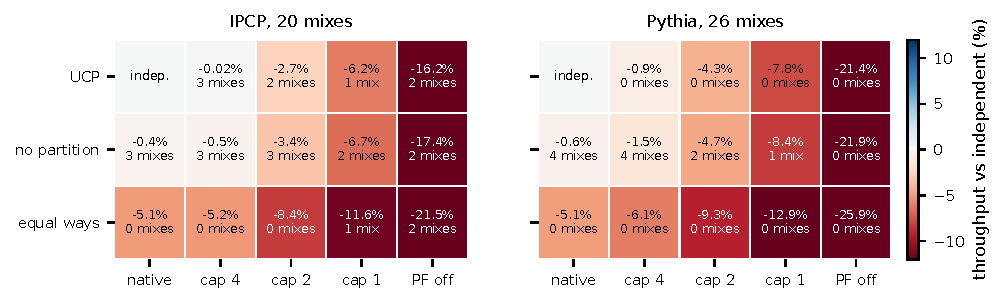
\includegraphics[width=0.92\textwidth]{grid_headroom.pdf}
\caption{Uniform knobs, 4-core: throughput of every combination of a degree cap applied to all cores and a
partitioning policy, relative to independent operation (UCP + native prefetcher, ``indep.''), geometric mean over
the mixes, and the number of mixes in which the configuration gains at least 2\%.  No uniform configuration beats
independent operation on average.}
\label{fig:grid}
\end{figure*}

\paragraph{Uniform knobs never beat independent operation}
In \cref{fig:grid} every cell is at or below independent operation: the best uniform configuration (degree cap 4
with UCP for IPCP, native Pythia without partitioning) is within 0.6\% of it, caps 2 and 1 lose 2.7--12.9\%,
switching prefetching off loses 16--26\%, and equal way allocation loses 5.1\% even with native prefetchers.  A
uniform cap also hurts fairness: the mean worst core of a mix drops to 0.98, 0.89 and 0.81 of its independent IPC
at caps 4, 2 and 1 (IPCP; Pythia 0.97, 0.90, 0.82).  A uniform configuration helps only in a few mixes (at most 4 of 20 or 26 per cell).  Even an oracle that picks the best uniform configuration per mix gains only
3.3\% (IPCP) and 0.4\% (Pythia); the IPCP mean is carried by a single mix (mix 9, +39\% with prefetching off)
in this one-channel setup.

\begin{table}[!htbp]
\centering
\caption{Headroom over independent PF+UCP (throughput).  Uniform knobs: best of the 15 configurations of
\cref{fig:grid} chosen per mix.  Per-core oracle: best validated per-core degree caps $\times$ way allocation.}
\label{tab:oracle}
\footnotesize
\resizebox{\columnwidth}{!}{\begin{tabular}{lllrccc}
\toprule
Search & Setup & PF & Mixes & Mean & Max & $\geq$+3\% \\
\midrule
Uniform knobs & 4-core, 1 ch. & IPCP & 20 & +3.3\% & +39.2\% & 4 \\
Uniform knobs & 4-core, 2 ch. & Pythia & 26 & +0.4\% & +6.0\% & 2 \\
\midrule
Per-core oracle & 4-core, 9.6\,GB/s & IPCP & 14 & +4.6\% & +17.2\% & 7 \\
Per-core oracle & 4-core, 9.6\,GB/s & Pythia & 14 & +1.1\% & +5.4\% & 2 \\
Per-core oracle & 8-core, 2.4\,GB/s & IPCP & 8 & +14.9\% & +38.2\% & 6 \\
\bottomrule
\end{tabular}
}
\end{table}

\begin{figure*}[!tp]
\centering
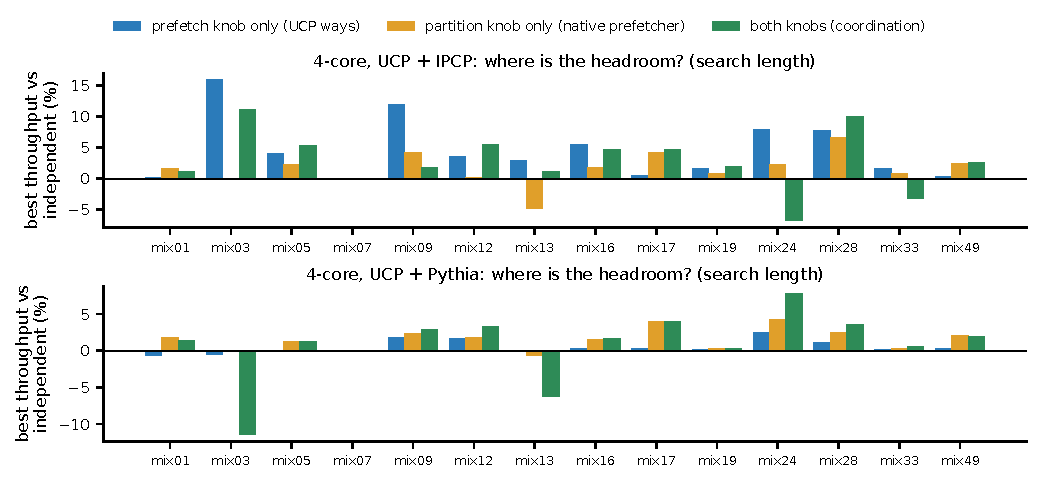
\includegraphics[width=0.9\textwidth]{oracle_knobs.pdf}
\caption{Per-core static oracle, 4-core, 9.6\,GB/s/core: where is the headroom?  Best throughput over independent
operation when only the prefetch knob (UCP keeps partitioning), only the partition knob (native prefetchers) or both
are searched, at the search length.  A missing bar: no configuration of that search was evaluated.}
\label{fig:oracle}
\end{figure*}

\begin{figure*}[!tp]
\centering
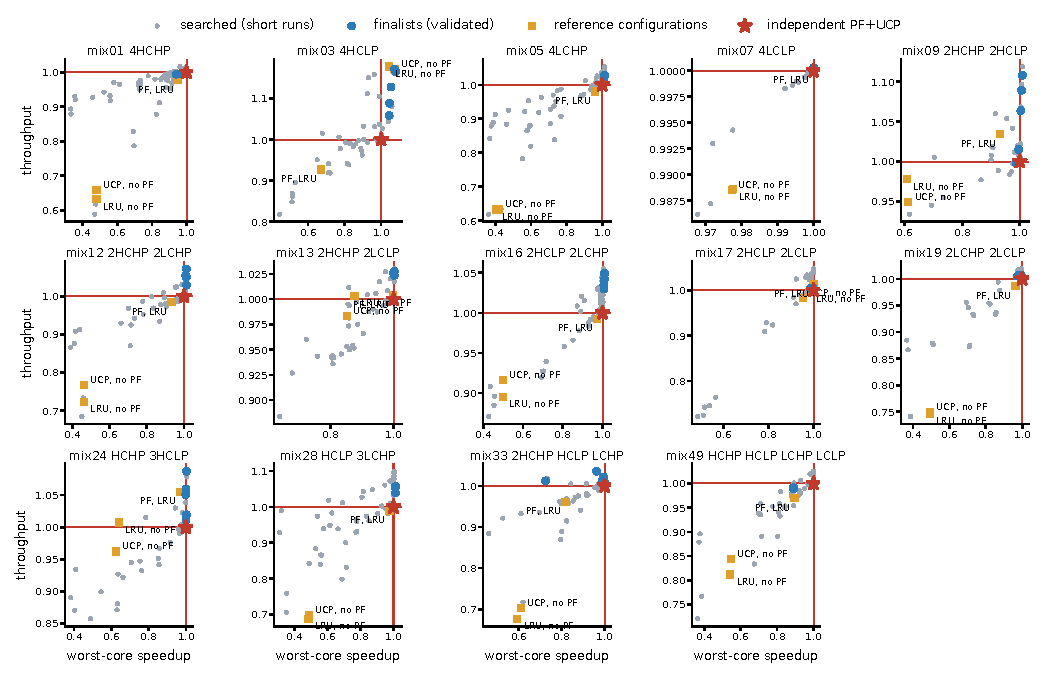
\includegraphics[width=0.9\textwidth]{oracle_scatter_ipcp.pdf}
\caption{Per-core static oracle, 4-core, 9.6\,GB/s/core, UCP+IPCP: every fixed configuration evaluated, as
throughput against the speedup of the worst core, both relative to independent operation (star).  Grey: searched
configurations (short runs); blue: finalists re-validated at full length; orange: prefetching alone on LRU, UCP alone
and neither.  Up and to the right of the star is better.}
\label{fig:scatter}
\end{figure*}
\paragraph{Per-core decisions find headroom with IPCP, and need both knobs}
Choosing a degree cap and a way allocation per core (\cref{tab:oracle}) finds \OrcIpMean\% (IPCP) and
\OrcPyMean\% (Pythia) on average after validation, at most \OrcMax\%, and at least 3\% in \OrcIpThree{} of \OrcIpN{}
IPCP mixes but only \OrcPyThree{} of \OrcPyN{} Pythia mixes.  \Cref{fig:scatter} (IPCP; Pythia in \cref{fig:scatterpy}, appendix) shows every configuration
the search evaluated.  With Pythia, the best validated configuration is within 1.5\% of independent operation in
12 of 14 mixes.  \Cref{fig:oracle} decomposes the search.  The two prefetchers need different knobs: for IPCP the prefetch knob alone is worth \KnIpPf\%
at the search length and the partition alone \KnIpPart\%, for Pythia, which already adapts to bandwidth, the partition is
worth more (\KnPyPart\% against \KnPyPf\%).  In \KnIpBoth{} (IPCP) and \KnPyBoth{} (Pythia) of the \KnIpN{} mixes the best configuration sets
\emph{both} knobs.  The joint search sometimes ends in a worse configuration than either single-knob search (\KnFragile), and part of the search-length gain disappears at full length (IPCP: \KnIpBest\% on \KnIpN{} mixes at
search length, \OrcIpMean\% on the \OrcIpN{} validated mixes).  On 4 cores with ample bandwidth the per-core oracle thus finds headroom mainly in the prefetch knob with IPCP and
in the partition with Pythia.

\subsection{Finding 2: with less bandwidth per core, prefetching creates casualties}
\label{sec:scale}

\begin{table}[!htbp]
\centering
\caption{8-core factorial study (20 mixes): throughput vs no prefetching and no partitioning, max slowdown,
fairness, and casualty cores (of 160).}
\label{tab:scaleup}
\footnotesize
\resizebox{\columnwidth}{!}{\begin{tabular}{llrcccc}
\toprule
DRAM & Configuration & PF & Thr. vs no-PF & Max slowdown & Fairness & Casualties \\
\midrule
2400 MT/s & No PF, no partitioning & -- & 1.000 & 2.02 & 0.57 & 0 \\
2400 MT/s & UCP only & -- & 1.004 & 2.03 & 0.57 & 23 \\
2400 MT/s & PF only (LRU) & IPCP & 1.220 & 2.05 & 0.42 & 45 \\
2400 MT/s & PF only (LRU) & Pythia & 1.309 & 1.89 & 0.43 & 33 \\
2400 MT/s & PF + UCP & IPCP & 1.221 & 2.11 & 0.41 & 47 \\
2400 MT/s & PF + UCP & Pythia & 1.307 & 1.79 & 0.44 & 32 \\
\midrule
1200 MT/s & No PF, no partitioning & -- & 1.000 & 2.18 & 0.55 & 0 \\
1200 MT/s & UCP only & -- & 1.003 & 2.20 & 0.55 & 25 \\
1200 MT/s & PF only (LRU) & IPCP & 1.134 & 2.48 & 0.40 & 61 \\
1200 MT/s & PF only (LRU) & Pythia & 1.234 & 2.27 & 0.41 & 42 \\
1200 MT/s & PF + UCP & IPCP & 1.129 & 2.53 & 0.39 & 57 \\
1200 MT/s & PF + UCP & Pythia & 1.231 & 2.14 & 0.43 & 41 \\
\bottomrule
\end{tabular}
}
\end{table}

\begin{figure*}[!tp]
\centering
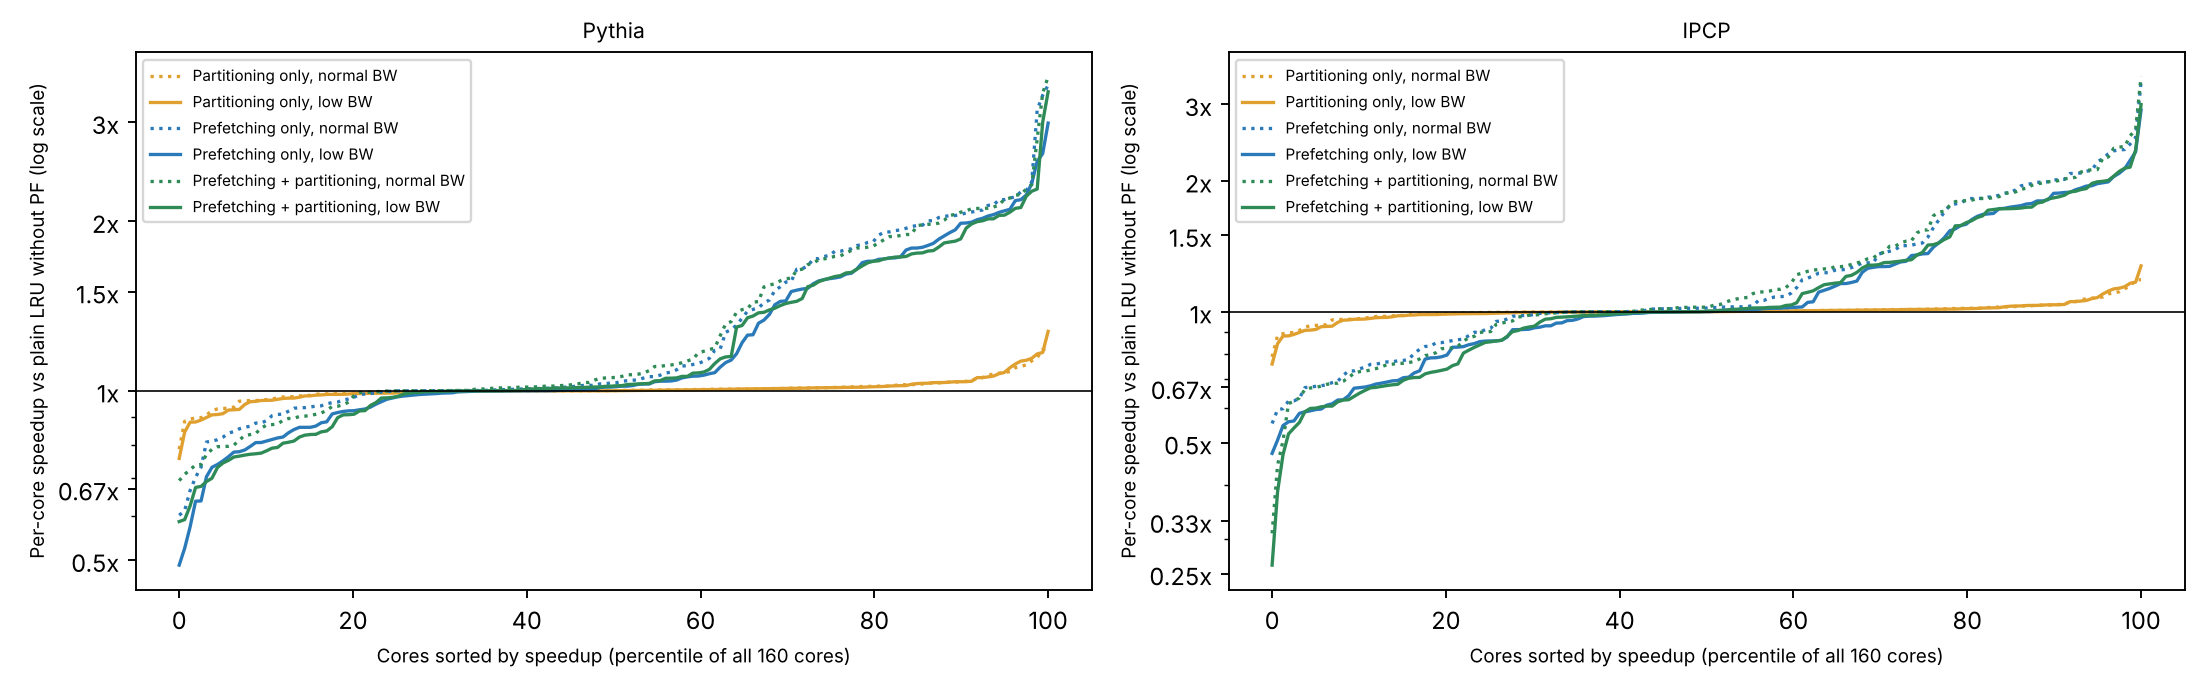
\includegraphics[width=0.8\textwidth]{percore_8core.png}
\caption{8-core: per-core speedup over plain LRU without prefetching for all 160 cores, sorted, for each mechanism
alone and both together, at 4.8 (dotted) and 2.4\,GB/s per core (solid).  The averages of
\cref{tab:scaleup} hide a left tail of cores that prefetching slows down, and the tail grows when the bandwidth per
core halves.}
\label{fig:casualties}
\end{figure*}

On 8 cores (\cref{tab:scaleup}, \cref{fig:casualties}), halving the per-core bandwidth from 4.8 to 2.4\,GB/s lowers
the throughput gain of IPCP+UCP from 22\% to 13\% and raises the casualties from 47 to 57 of 160 cores (Pythia: 32 to
41); with IPCP the worst core of a mix is slowed down 2.5$\times$ on average.  The per-core static oracle at 2.4\,GB/s per core
finds a mean headroom of 14.9\% and a maximum of 38.2\% for IPCP, at least 3\% in 6 of 8 mixes (\cref{tab:oracle};
every configuration in \cref{fig:scatter8}, appendix).  It comes almost entirely from the prefetch knob: at the
search length, tuning only the degrees reaches 19.8\% on average, tuning only the partition 4.4\%, and the joint
search, which evaluated only 16 configurations (against 144 and 88), $-2.4\%$.  In four of eight mixes the best
fixed configuration turns IPCP off on every core, which costs the worst core up to 54\%; the fairest configuration
that does not lose throughput throttles a single core in six of eight mixes and still gains 0.1--22\%.

\subsection{Finding 3: UCP barely reacts, and rewards the wrong prefetchers}

\begin{figure*}[!tp]
\centering
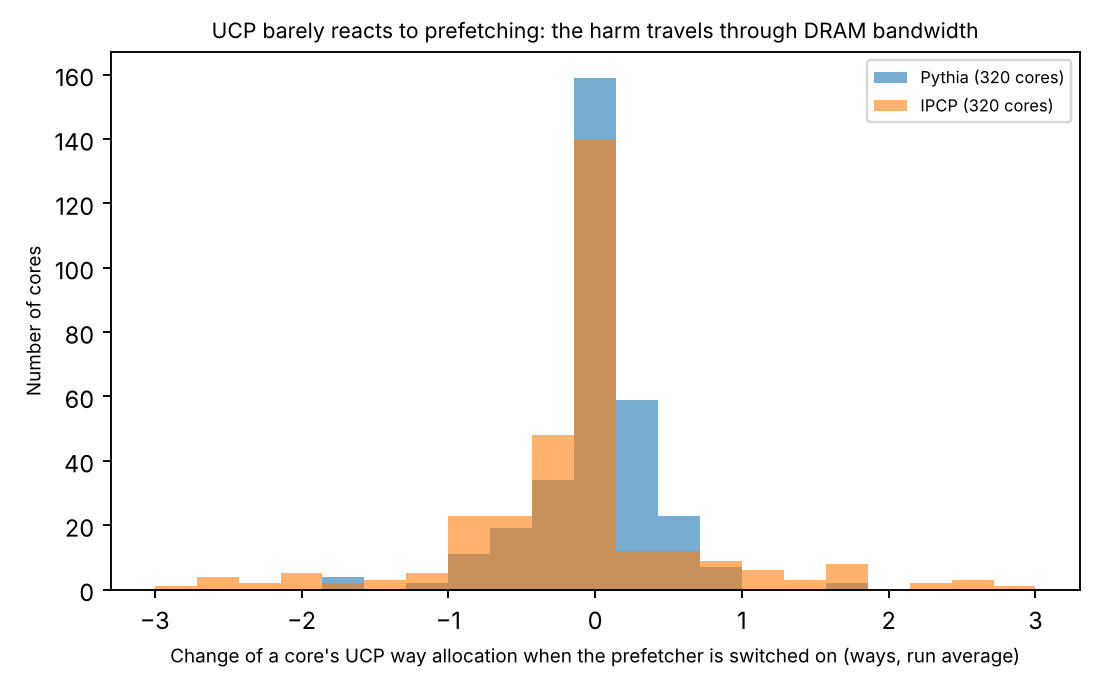
\includegraphics[height=1.75in]{realloc_8core.png}\hfill
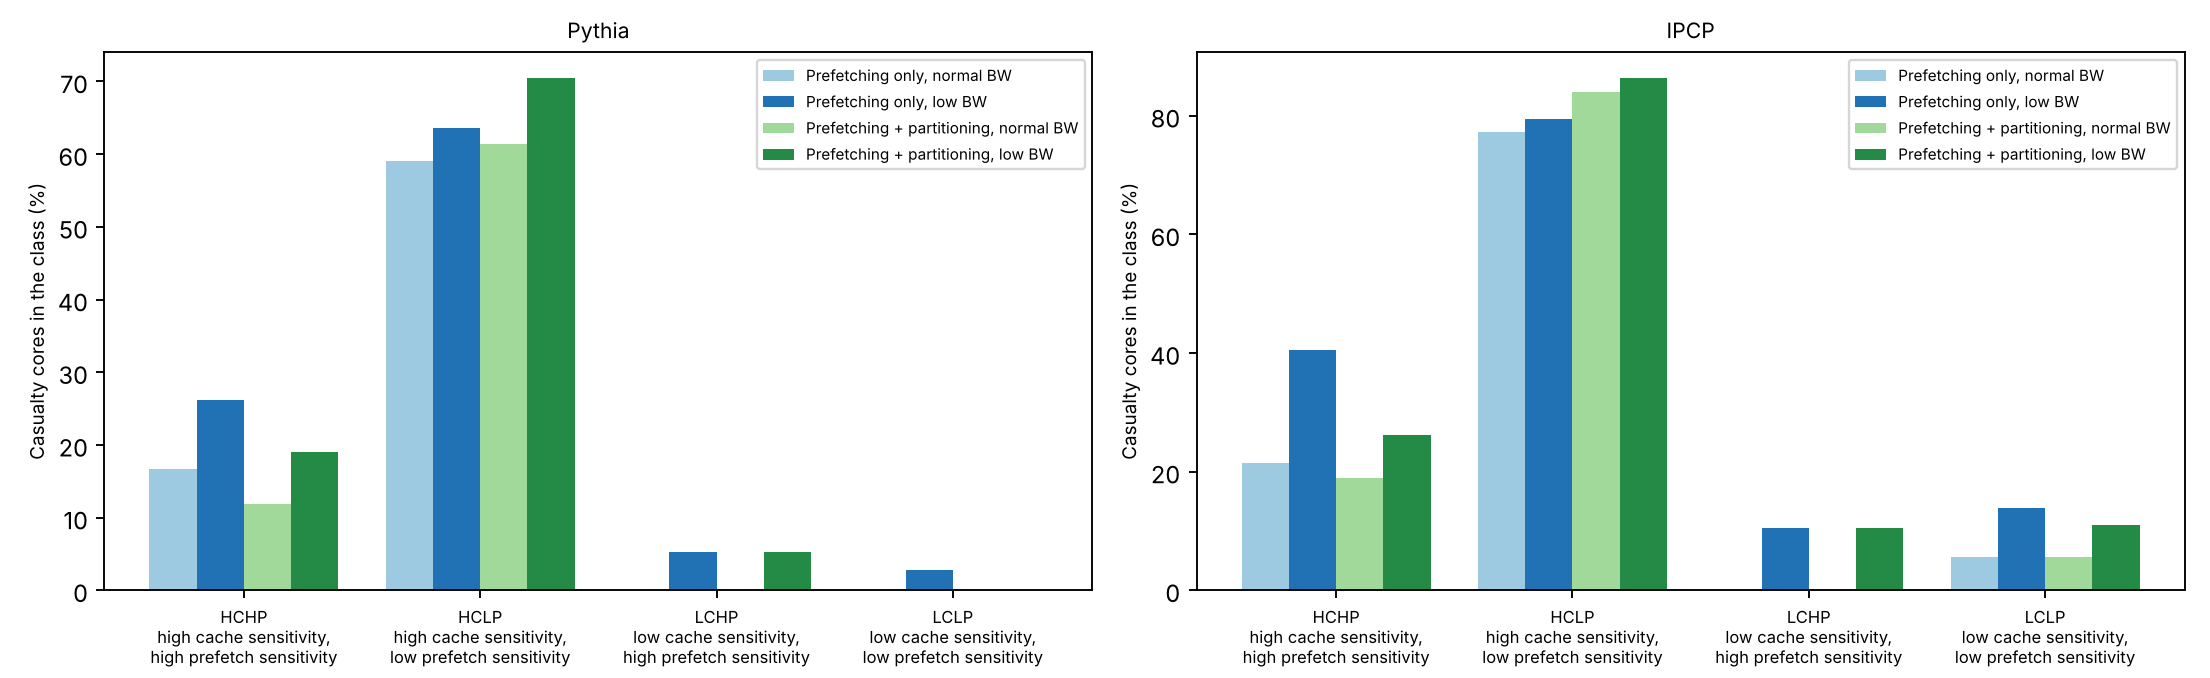
\includegraphics[height=1.75in]{byclass_8core.png}
\caption{8-core: change of each core's UCP way allocation when its prefetcher is switched on (left) and casualties by
workload class (right).
UCP changes the allocation of few cores; the casualties are mostly cache-sensitive (HC) cores.}
\label{fig:interaction}
\end{figure*}

Enabling the prefetcher changes the average UCP allocation of a core by at least one way for only 54 of 320
(IPCP) and 8 of 320 (Pythia) cores (\cref{fig:interaction}, left).
Where UCP does react, it reacts the wrong way: with IPCP, the 31 cores that gain at least one way have a median
prefetch accuracy of 0.08 (against 0.29 over all cores), and all 23 cores that lose at least one way are
cache-sensitive (15 HCLP, 8 HCHP).  The casualties concentrate in exactly these classes (\cref{fig:interaction},
right).  In 39--49\% (IPCP) and 33--41\% (Pythia) of the cores, enabling both mechanisms is worse than the better of
the two alone.

\subsection{Finding 4: why prior-style throttling loses throughput}

\begin{figure*}[!tp]
\centering
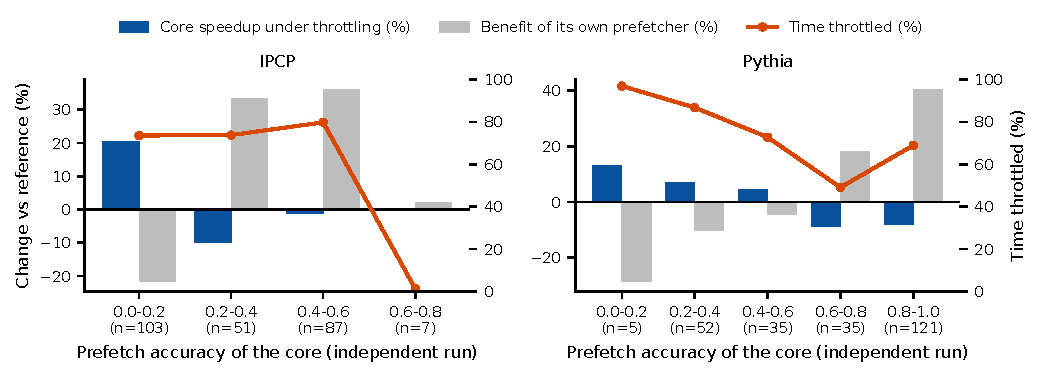
\includegraphics[width=0.9\textwidth]{root_cause_accuracy.pdf}
\caption{Fairness-driven throttling (FDT: keep a throttle step when the fairness score improves), 4-core 2.4\,GB/s/core
and 8-core cores grouped by their prefetch accuracy.  Blue: the core's speedup under FDT over independent operation; grey: the
core's speedup in the independent run over neither prefetching nor partitioning; line: share of time FDT kept it
throttled.  On average the inaccurate cores (accuracy below about 0.2 for IPCP, 0.6 for Pythia) gain and the accurate
ones lose.}
\label{fig:rootcause}
\end{figure*}

We implemented a feedback throttling controller in the spirit of HPAC~\cite{ebrahimi2009hpac}, which we call
\emph{fairness-driven throttling} (FDT): every epoch it
detects DRAM pressure, tentatively lowers the prefetch level of the core with the most useless (or the most) prefetch
traffic, and keeps the step if the weighted harmonic mean of all cores' IPC improves.  It gains up to 41\% on some mixes
(+28\%, +36\% and +41\% on three 8-core IPCP mixes), but loses up to 11.5\% on a 4-core mix and 15.7\% on an 8-core
mix, with 5 of 22 4-core mixes below $-2\%$ for IPCP and 7 for Pythia.  \Cref{fig:rootcause} groups the cores by
prefetch accuracy: on average the inaccurate cores (accuracy below 0.2 for IPCP, 0.6 for Pythia) gain and the
accurate ones lose.  The cores that the independent run speeds up by at least 1.3$\times$ over neither mechanism (71 with IPCP, 88
with Pythia) are
kept throttled 93\% and 88\% of the time and end up 11\% and 16\% slower.  FDT keeps a step only when the fairness
score of the trial rises, so these steps passed its test although they slowed the throttled cores down.  Coordinating the partition as well (FDT+PSR, FDT+Reclaim) did not remove these losses: all three designs have 5
4-core IPCP mixes below $-2\%$ (\cref{tab:final4}).  Changing the acceptance rule did: TSC-T, which differs from FDT
mainly in its acceptance rule, has 2 such mixes.

\subsection{Problem statement}
\label{sec:statement}

Running the two mechanisms independently has three problems:
\begin{enumerate}
  \item \textbf{Prefetching slows down more cores when bandwidth per core is low.}  On 8 cores, halving the bandwidth
        per core from 4.8 to 2.4\,GB/s raises the casualties (cores more than 2\% slower than with neither prefetching
        nor partitioning) from 47 to 57 of 160 with IPCP and from 32 to 41 with Pythia (\cref{tab:scaleup}).
  \item \textbf{UCP gives ways to inaccurate prefetchers.}  UCP's monitors count every hit, including hits on
        prefetched lines~\cite{qureshi2006ucp}.  With IPCP, the cores that gain ways when prefetching is enabled have
        a median prefetch accuracy of 0.08 (0.29 over all cores), and all cores that lose ways are cache-sensitive
        (Finding~3).
  \item \textbf{Fixing one side is not enough.}  None of the 14 uniform settings of the two knobs beats independent
        operation, and degree caps of 2 or 1 lose 2.7--12.9\% (\cref{fig:grid}).  Throttling on fairness alone (FDT)
        keeps the cores that prefetching speeds up by at least 1.3$\times$ throttled about 90\% of the time; they end
        up 11--16\% slower (Finding~4, \cref{fig:rootcause}).
\end{enumerate}

\paragraph{Why two-way}
The per-core oracle (\cref{fig:oracle}, \cref{sec:headroom}) gains \KnIpPf\% (IPCP) and \KnPyPf\% (Pythia) when it
searches only the prefetch knob and \KnIpPart\% and \KnPyPart\% when it searches only the partition.  In \KnIpBoth{}
(IPCP) and \KnPyBoth{} (Pythia) of \KnIpN{} mixes the best setting it finds changes both knobs.

\paragraph{Problem}
\emph{Coordinate prefetch throttling and LLC partitioning in both directions under limited DRAM bandwidth, so that
throughput and fairness increase by removing only the prefetching that does not help its own core and by not giving
LLC ways to useless prefetches, without lowering the overall throughput.}  The controller should work with any prefetcher and any way partitioner without changing them.

\section{Methodology: a Throughput-Safe Coordinator}
\label{sec:method}

\begin{figure*}[!tp]
\centering
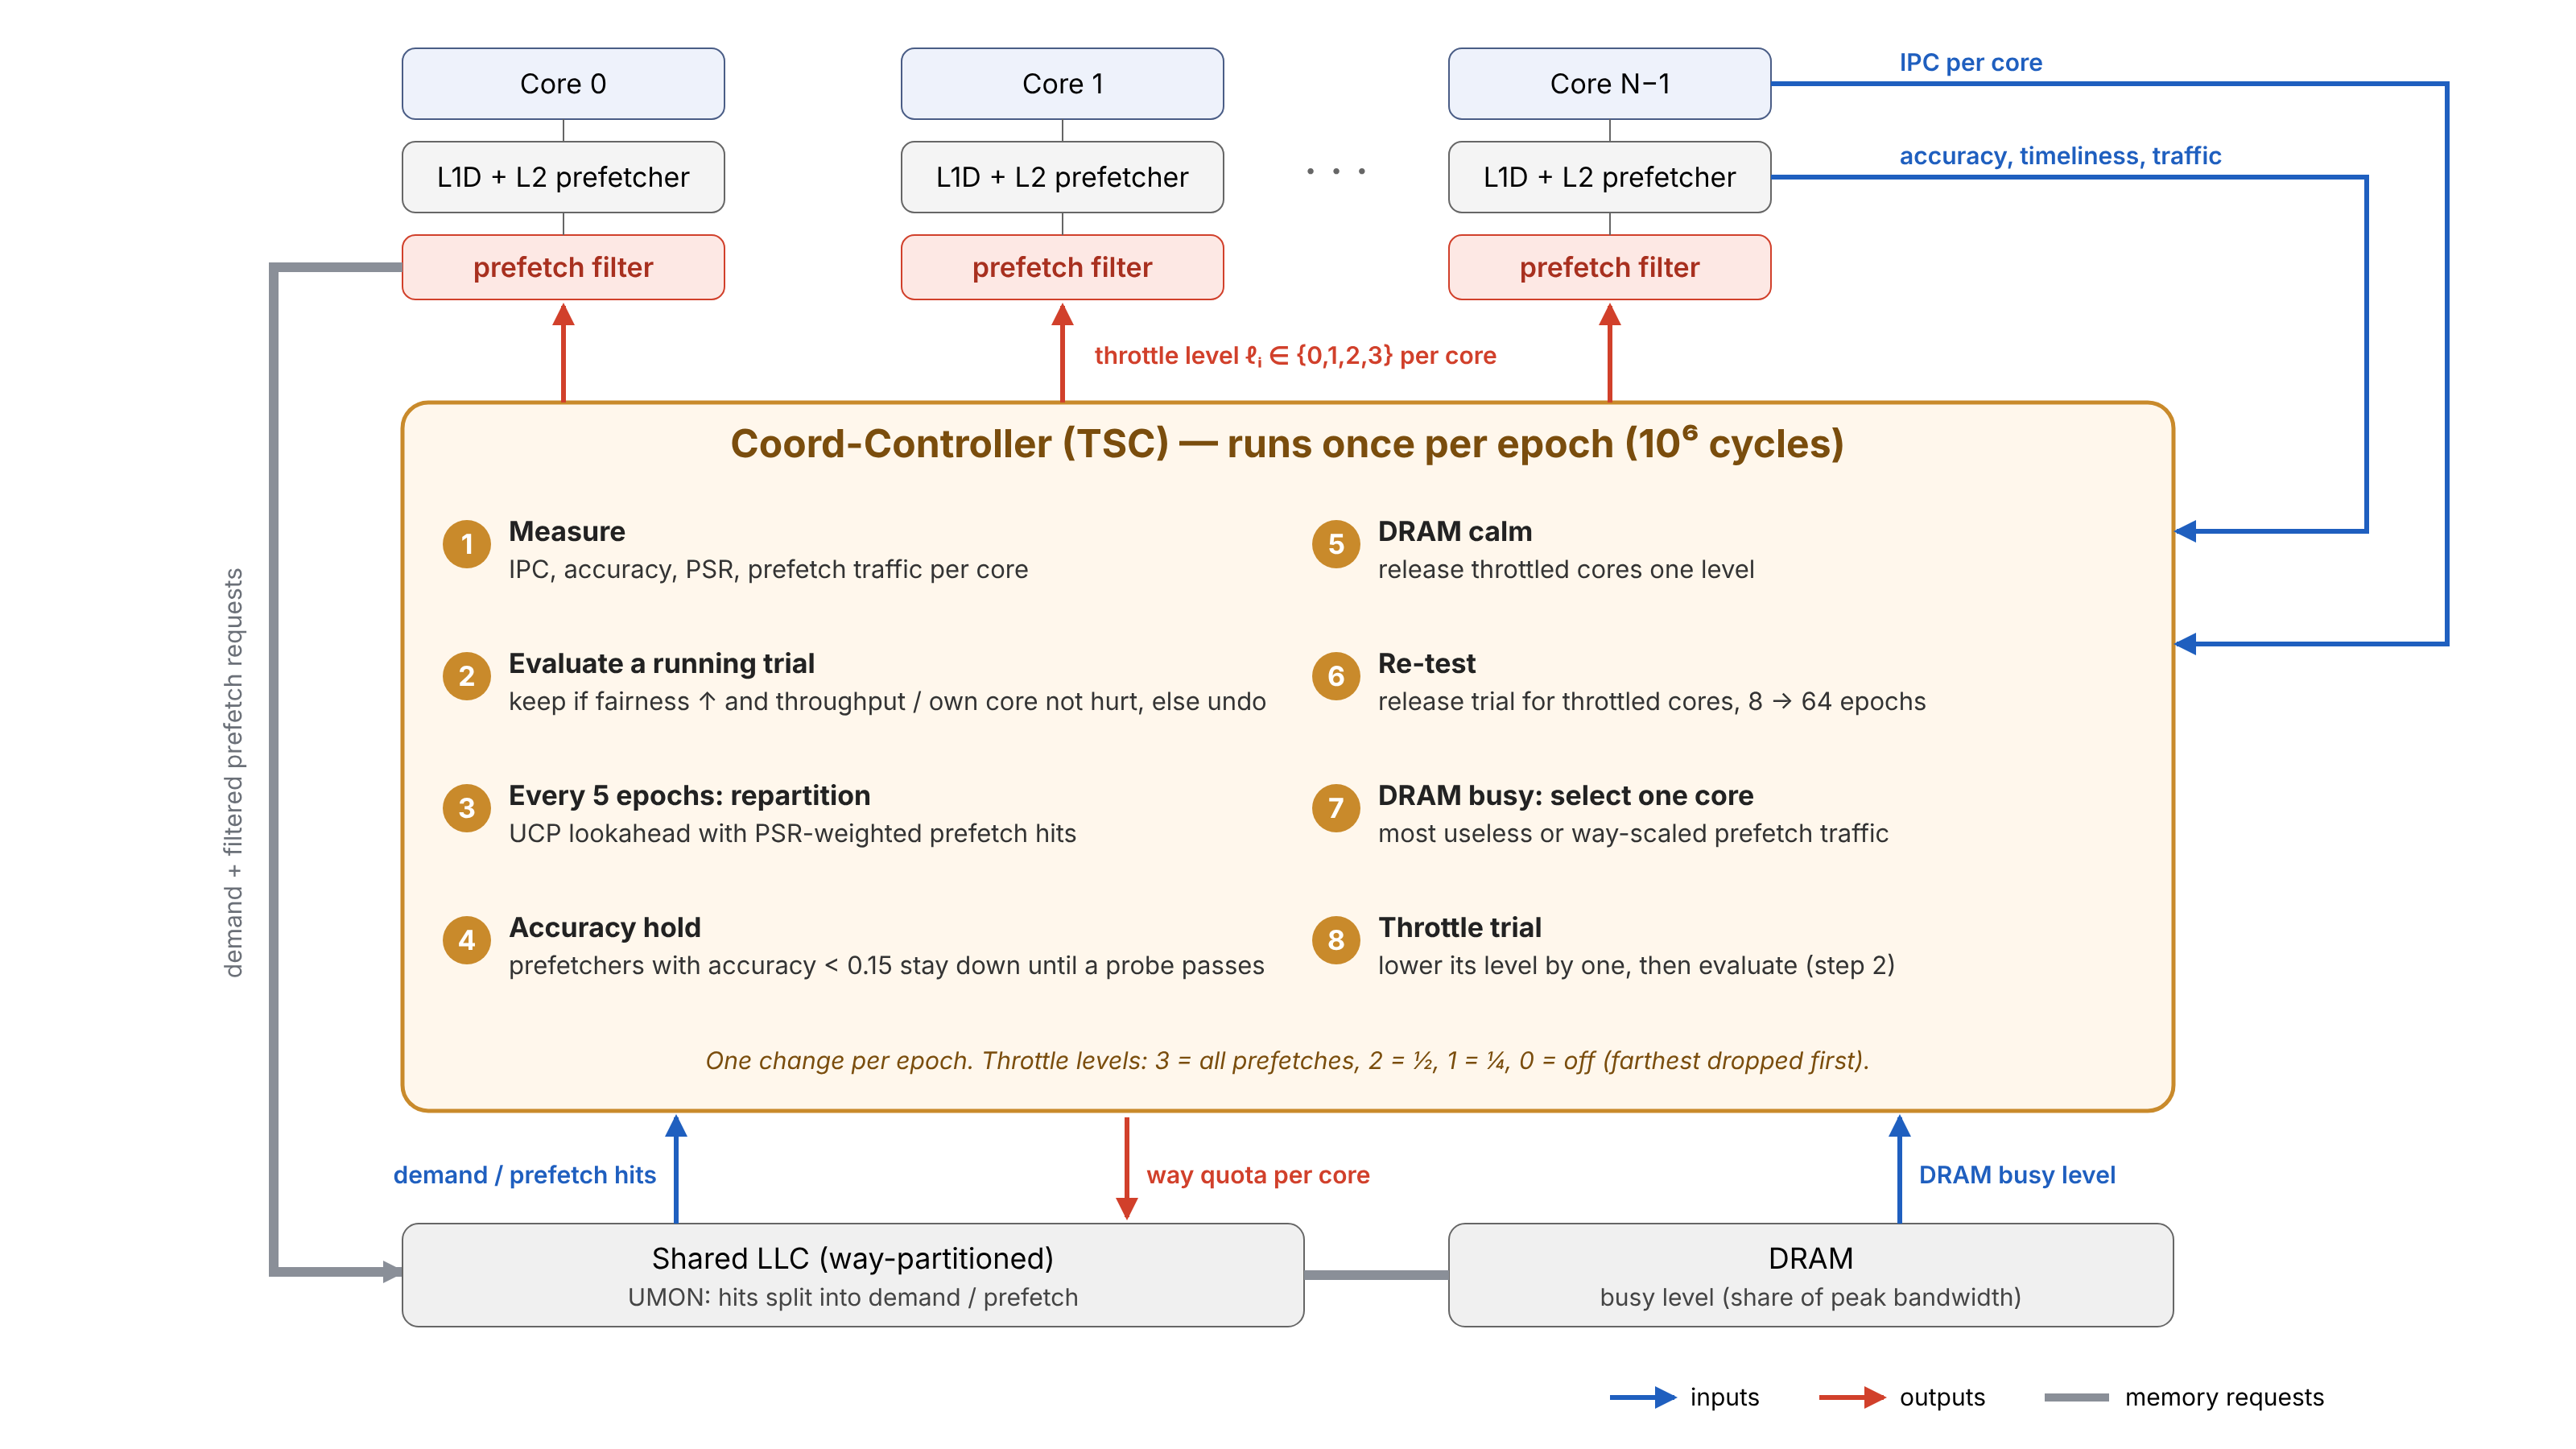
\includegraphics[width=0.92\textwidth]{tsc_overview.png}
\caption{TSC overview.  Once per epoch the coordinator reads per-core IPC, prefetch accuracy, timeliness and
traffic, UCP's demand and prefetch hits and the DRAM busy level (blue), and sets a throttle level per core, applied by
a prefetch filter that drops the farthest requests first, and the per-core LLC way quota (red).}
\label{fig:controller}
\end{figure*}

\Cref{fig:controller} gives an overview.  The coordinator is a small finite-state controller that runs once per epoch
of $10^6$ cycles.  It does not modify the prefetchers, and from UCP it needs only split hit counters and an interface to set the
way quota (\cref{sec:knobs}).  It acts through two interfaces: a \emph{prefetch filter} that lets only part of a core's prefetch requests
through (\cref{sec:knobs}), and the LLC way quota of each core.

\subsection{What the coordinator measures}
\begin{itemize}
  \item \textbf{Per-core prefetch quality} from the private L1D and L2: prefetches filled, \emph{useful} (first
        demand hit on a prefetched block), \emph{late} (demand merged with an in-flight prefetch) and \emph{useless}
        (evicted unused).  Accuracy $a=\text{useful}/(\text{useful}+\text{useless})$, timeliness
        $t=\text{useful}/(\text{useful}+\text{late})$ and the prefetch success rate $\mathit{PSR}=a\cdot t$ are kept as
        exponentially weighted averages.  A request that the prefetch filter drops never reaches the cache, so it is
        never counted as useful, useless or late: the metrics describe only the prefetches that were actually sent.
  \item \textbf{Per-core prefetch DRAM traffic}: LLC prefetch misses per kilo-cycle, and its useless part
        $(1-a)\times$traffic.
  \item \textbf{Per-core IPC} of the epoch, and an exponentially weighted reference IPC.
  \item \textbf{DRAM pressure}: how busy DRAM is, as the share of its peak bandwidth in use, reported in four
        levels numbered 0--3 (below 25\%, 25--50\%, 50--75\%, above 75\%) and averaged over the epoch.  DRAM counts as
        \emph{busy} when this average is above 1.5 (i.e.\ mostly in the upper two levels) and as \emph{calm} when it
        is below.
  \item \textbf{Partition state}: each core's way quota and UCP's sampled shadow-tag hit counters, which we split
        by request type into demand hits $h^d_c[r]$ and prefetch hits $h^p_c[r]$ per LRU position $r$.
\end{itemize}

\subsection{What the coordinator controls}
\label{sec:knobs}
\paragraph{Prefetch filter (farthest requests dropped first)}
Each core has a \emph{throttle level} that sets which share of its prefetch requests is sent:
\begin{center}\footnotesize
\begin{tabular}{lcccc}
\toprule
Throttle level $\ell$ & 3 & 2 & 1 & 0 \\
Share of requests sent $f$ & all & 1/2 & 1/4 & none \\
\bottomrule
\end{tabular}
\end{center}
Level 3, the default, leaves the prefetcher untouched; level 0 switches it off.  \emph{Throttling} a core means lowering its level by one; \emph{releasing} it means raising it by one.  Every
prefetcher sends its requests through one function per cache (\texttt{prefetch\_line}), and the filter sits there.
When a prefetcher is triggered by a demand access, it issues several requests at once, nearest address first (stride,
stream and offset prefetchers all do so); we call these requests a \emph{burst}.  The filter lets the first
share $f$ of each burst through and drops the rest, i.e.\ the farthest, least timely ones.  Example: a prefetcher with
degree 4 issues the lines $+1,+2,+3,+4$ ahead; at level 2 only $+1$ and $+2$ are sent, at level 1 only $+1$.  Because
burst sizes vary, the filter uses the running average burst size $\bar B$ and carries the fraction left over from one
burst to the next, so that a prefetcher issuing one request per trigger is thinned to every second or fourth request.
No prefetcher code is changed.
\paragraph{LLC way quota}
Through five functions (read quota, set quota, enable external control, read and age the split hit counters) the
coordinator replaces UCP's own repartitioning.  We implemented them for UCP only.

\subsection{Prefetch control}

\begin{figure*}[!tp]
\centering
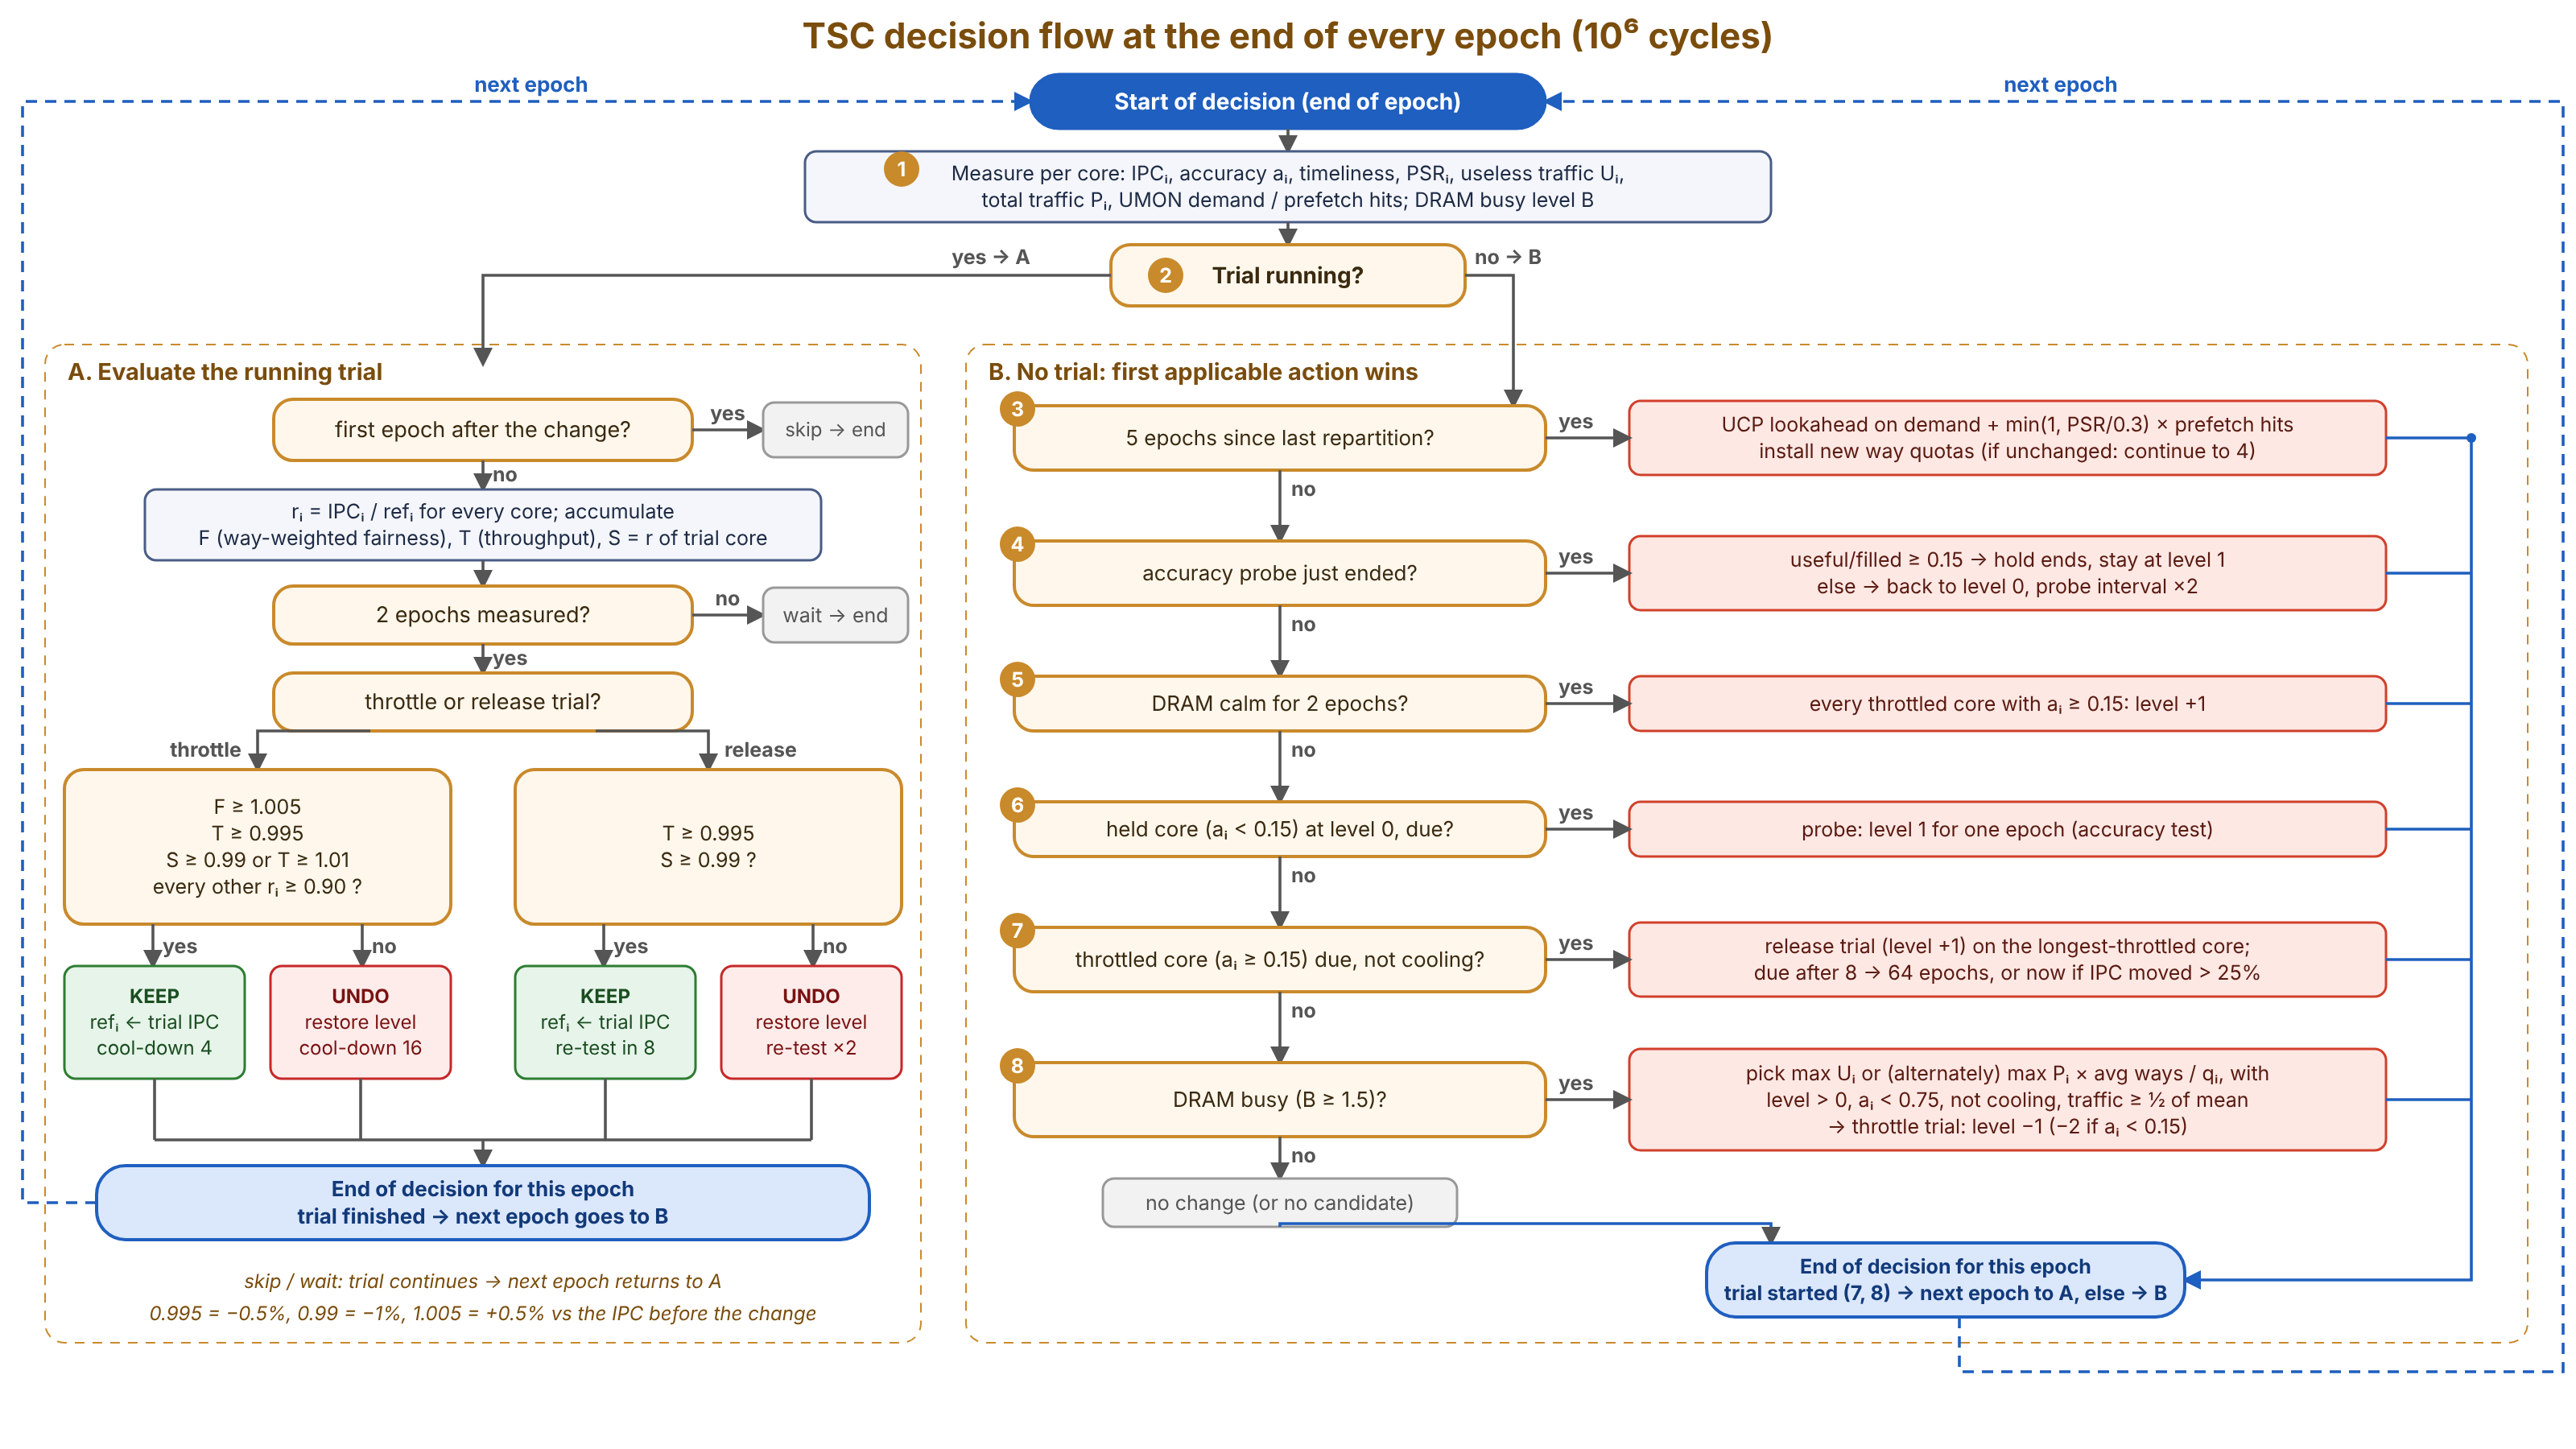
\includegraphics[width=0.95\textwidth]{tsc_flowchart.png}
\caption{TSC decision flow at the end of every epoch.  A running trial is evaluated in A; otherwise the first
applicable action of B is taken.  Every path ends the decision for the epoch; a trial started in B is evaluated in A
in the following epochs, and a finished trial returns control to B.}
\label{fig:flow}
\end{figure*}

\begin{algorithm}[!tp]
\caption{TSC: decision at the end of every epoch.  The functions are in Algorithm~\ref{alg:funcs}, the constants in
\cref{tab:params}.}
\label{alg:epoch}
\small
\DontPrintSemicolon
\SetKwProg{Fn}{Function}{}{end}
\SetKwFunction{FEnd}{EndOfEpoch}\SetKwFunction{FTrial}{Trial}\SetKwFunction{FEval}{Evaluate}
\SetKwFunction{FSel}{SelectCore}\SetKwFunction{FHeld}{Held}\SetKwFunction{FPart}{Repartition}
\SetKwFunction{FProbe}{EndProbe}
\KwIn{per core $i$: $\mathit{IPC}_i$, prefetch accuracy $a_i$ and success rate $\mathit{PSR}_i$, useless and
  total prefetch traffic $U_i$, $P_i$, way quota $q_i$; DRAM busy level $B$}
\KwOut{throttle level $\ell_i\in\{0,1,2,3\}$ and way quota $q_i$ of every core}
\KwData{$\mathit{ref}_i$: reference IPC of core $i$ (its IPC before a change)}
\BlankLine
\Fn{\FEnd{}}{
  \lIf(\tcp*[f]{measure, keep or undo}){a trial is running}{\FEval{}; \Return}
  \lIf(\tcp*[f]{PSR-weighted UCP}){every $E_q$ epochs}{\FPart{}}
  \lIf(\tcp*[f]{held core probed}){a probe has ended}{\FProbe{}; \Return}
  \If(\tcp*[f]{no pressure: give back}){DRAM calm for $C$ epochs}{
    $\ell_i\gets\ell_i+1$ for every throttled $i$ with $\neg$\FHeld{$i$}; \Return
  }
  \lIf(\tcp*[f]{probe}){a held core $i$ at level 0 is due}{$\ell_i\gets1$ for one epoch; \Return}
  \lIf(\tcp*[f]{re-test}){a throttled core $i$ with $\neg$\FHeld{$i$} is due}{\FTrial{$i$, $+1$}; \Return}
  \If(\tcp*[f]{pressure}){$B\ge B_{hi}$}{
    $j\gets$\FSel{}\;
    \lIf{$j\neq\bot$}{\FTrial{$j$, $-2$ \textbf{if} $a_j<a_2$ \textbf{else} $-1$}}
  }
}
\end{algorithm}

\begin{algorithm}[!tp]
\caption{Functions of TSC.}
\label{alg:funcs}
\small
\DontPrintSemicolon
\SetKwProg{Fn}{Function}{}{end}
\SetKwFunction{FTrial}{Trial}\SetKwFunction{FEval}{Evaluate}\SetKwFunction{FFilter}{Filter}
\SetKwFunction{FSel}{SelectCore}\SetKwFunction{FHeld}{Held}\SetKwFunction{FPart}{Repartition}
\SetKwFunction{FProbe}{EndProbe}
\Fn(\tcp*[f]{on every prefetch burst of core $i$}){\FFilter{$i$, burst}}{
  send the nearest share $f(\ell_i)$ of the burst; drop the rest \tcp*[r]{$f=0,\frac14,\frac12,1$}
}
\BlankLine
\Fn{\FHeld{$i$}}{\Return $a_i<a_{\mathit{hold}}$ \tcp*[r]{no release trial, no calm release}}
\BlankLine
\Fn{\FSel{}}{
  $x_i\gets U_i$, or (alternately) $x_i\gets P_i\cdot\bar q/q_i$ \tcp*[r]{useless / way-scaled traffic}
  \Return $\arg\max x_i$ over cores with $\ell_i>0$, $a_i<a_{\mathit{prot}}$, not cooling down\;
}
\BlankLine
\Fn{\FTrial{$j$, $\delta$}}{
  $\ell_j\gets\ell_j+\delta$; skip 1 epoch, then measure $K$ epochs \tcp*[r]{then \FEval}
}
\BlankLine
\Fn{\FEval{}}{
  $r_i\gets\mathit{IPC}_i/\mathit{ref}_i$ for every core\;
  $F\gets$ way-weighted harmonic mean of $r_i$;\ $T\gets$ mean of $r_i$;\ $S\gets r_j$\;
  \eIf(\tcp*[f]{throttle trial}){$\delta<0$}{
    $\mathit{ok}\gets F\ge1+g\ \wedge\ T\ge1-\tau_T\ \wedge\ (S\ge1-\tau_S\ \vee\ T\ge1+\tau_W)$
      $\wedge$ no other $r_i<1-\tau_V$\;
  }(\tcp*[f]{release trial}){
    $\mathit{ok}\gets T\ge1-\tau_T\ \wedge\ S\ge1-\tau_S$\;
  }
  \lIf{$\mathit{ok}$}{$\mathit{ref}_i\gets$ IPC measured in the trial}
  \lElse{$\ell_j\gets\ell_j-\delta$; core $j$ cools down}
}
\BlankLine
\Fn{\FProbe{}}{
  $a\gets$ useful / filled prefetches of the probed core $i$ in the probe epoch\;
  \lIf(\tcp*[f]{hold ends}){$a\ge a_{\mathit{hold}}$}{keep $\ell_i=1$}
  \lElse{$\ell_i\gets0$}
}
\BlankLine
\Fn{\FPart{}}{
  $w_i\gets\min(1,\ \mathit{PSR}_i/\mathit{PSR}_{\mathit{full}})$\;
  $q\gets$ UCP lookahead on demand hits $+\ w_i\cdot$ prefetch hits\;
}
\end{algorithm}

\Cref{fig:flow} shows the decision flow, and Algorithms~\ref{alg:epoch} and~\ref{alg:funcs} give it as pseudocode.  Its design follows directly from the findings of
\cref{sec:problem}.  The central mechanism is the \emph{trial}: the controller never decides from a model whether a
change will help.  It makes one small change (one core, one level), measures its effect on every core for a few
epochs, and keeps the change only if the measurement passes the acceptance test below; otherwise it restores the
previous level.  A \emph{throttle trial} lowers a core's level by one, a \emph{release trial} raises it by one.

\paragraph{One change at a time, measured}
When DRAM is busy, the controller picks the core to throttle by alternating between two rankings.  The first
ranks cores by their \emph{useless} prefetch traffic, i.e.\ prefetched lines that are evicted unused: they use DRAM bandwidth and cache space without
benefit.  The second ranks cores
by their total prefetch traffic, scaled by the average way quota divided by the core's own quota, i.e.\ the cores
that send the most prefetch traffic to DRAM although UCP gives them few ways (UCP's monitors say they gain little
from cache space).  The top candidate gets a throttle trial.  A trial does not score the first epoch after the change and scores the next two.

\paragraph{Throughput-safe acceptance}
Each core $i$ keeps a reference IPC, $\mathit{ref}_i$: an exponentially weighted average of its IPC in the epochs
before the trial.  During the trial its speedup is $r_i=\mathit{IPC}_i/\mathit{ref}_i$.  We compare ratios rather than
raw IPC because the IPC of the cores of a mix differs by up to $15.6\times$ in our 4-core runs (median $5.5\times$).  A sum of IPCs would be dominated by the
fast cores: with IPCs of 1.6 and 0.2, a 5\% speedup of the fast core outweighs a 20\% slowdown of the slow one.  The ratio counts every core's relative change equally, as the weighted speedup does.
From the ratios the controller computes
\[
  T = \frac{1}{N}\sum_{i=1}^{N} r_i, \qquad
  F = \frac{\sum_i w_i}{\sum_i w_i/r_i},
\]
where $w_i = 1 + q_i/\bar q$, with $q_i$ the way quota of core $i$ and $\bar q$ the average quota (16 ways divided
by the number of cores).  $T$ and $F$ are computed for each of the two scored epochs and averaged.
$T$, the arithmetic mean, is the trial's throughput (normalised weighted speedup).  $F$, the harmonic mean, is
dominated by the smallest ratios, so it rises when a slowed-down core recovers; we call it the \emph{way-weighted fairness}.  Weighting it by
the way quota gives more weight to the cores to which UCP gives more ways; with IPCP, the casualties are mostly
cache-sensitive cores (\cref{fig:interaction}).  A throttle trial
is kept only if (i)~the way-weighted fairness $F$ rises by at least the gain $g=0.5\%$, (ii)~$T$ drops by at most 0.5\%, (iii)~the throttled
core itself loses at most 1\% unless $T$ rises by at least 1\%, and (iv)~no other core loses more than 10\%.  A
release trial is kept if $T$ and the released core do not lose more than 0.5\% and 1\%.  Rule~(iii) is the main difference to FDT.  On 4 cores at 2.4\,GB/s per core, the cores that the independent run
speeds up by at least 1.3$\times$ are throttled 39\% (IPCP) and 9\% (Pythia) of the time under \vthree{}, against
90\% and 82\% under FDT, and end up $+2.4\%$ and $-0.4\%$ instead of $-13.7\%$ and $-12.0\%$.

\paragraph{Gradual, periodically re-justified throttling}
Prefetching is the default.  A level is never removed or restored in one jump: each level is its own trial.  Every
throttled core is \emph{revalidated}: after 8 epochs it gets a release trial, which is kept unless throughput or the
core itself suffers.  A rejected revalidation doubles the interval, up to 64 epochs, and a phase change (the core's IPC
moved by more than 25\%) resets it.  When DRAM is calm for two epochs, every throttled core gets one level back.

\paragraph{Accuracy hold}
A throttled core whose accuracy is below 0.15 receives no release trial and is not released when DRAM is calm.
On 4 cores at 2.4\,GB/s per core, none of the 26 cores with an accuracy below 0.15 runs more than 2\% faster with both
mechanisms than with neither (at 9.6\,GB/s, 4 of 26 do; \cref{sec:limits}).  Adding the hold raises throughput from
4.6\% to 7.1\% (IPCP, \cref{tab:final4}).
At level 0 it issues no prefetches, so its accuracy is probed: one unjudged epoch at level 1, judged by
useful/filled prefetches of that epoch (both counted immediately, unlike evictions); only an accuracy of at least
0.15 ends the hold.

\subsection{Partition control}
Every five epochs (UCP's own interval) the coordinator computes the allocation with UCP's lookahead algorithm on the
utility
\[
  u_c[r] = h^d_c[r] + w_c\, h^p_c[r], \qquad w_c=\min\!\left(1,\ \mathit{PSR}_c/0.3\right),
\]
and installs it directly, without a trial.  A core whose prefetches are accurate and timely ($\mathit{PSR}\ge0.3$)
keeps exactly the ways UCP would give it, since UCP counts demand and prefetch hits alike; for a core with
$\mathit{PSR}<0.3$ the prefetch hits count only in proportion to its PSR.  The coordination thus works in both
directions: prefetch quality sets the partition's utility, and the way quota enters the throttling through the
way-weighted fairness $F$ and the way-scaled traffic ranking.

\subsection{Parameters and cost}

\begin{table}[!htbp]
\centering
\caption{Coordinator parameters (sensitivity in \cref{sec:sweep}).}
\label{tab:params}
\footnotesize
\resizebox{\columnwidth}{!}{\begin{tabular}{llr}
\toprule
Symbol & Meaning & Value \\
\midrule
$N$, $Q$ & cores, LLC ways & 4 or 8, 16 \\
-- & epoch length & $10^6$ cycles \\
$E_q$ & partition period & 5 epochs \\
$K$ & scored epochs per trial (after 1 skipped) & 2 \\
$\alpha$ & EWMA weight of the reference IPC & 0.3 \\
$B_{hi}$ & DRAM busy threshold (level 0--3) & 1.5 \\
$C$ & calm epochs before a release & 2 \\
$g$ & way-weighted fairness gain & 0.5\% \\
$\tau_T$ & throughput budget & 0.5\% \\
$\tau_S$ & own-core budget & 1\% \\
$\tau_W$ & throughput gain that overrides $\tau_S$ & 1\% \\
$\tau_V$ & victim guard (any other core) & 10\% \\
$a_{\mathit{prot}}$, $a_2$, $a_{\mathit{hold}}$ & protect / two-level drop / hold accuracy & 0.75 / 0.15 / 0.15 \\
$\sigma$ & minimum share of the mean traffic to be a candidate & 0.5 \\
$R_0$, $R_{\max}$ & revalidation interval, back-off limit & 8, 64 epochs \\
$\varphi$ & phase change (IPC change since last level change) & 25\% \\
$c_{\mathit{keep}}$, $c_{\mathit{rev}}$ & cool-down after a kept / reverted trial & 4, 16 epochs \\
$\mathit{PSR}_{\mathit{full}}$ & PSR for full prefetch credit in the UMON & 0.3 \\
\bottomrule
\end{tabular}}
\end{table}

\Cref{tab:params} lists the parameters.  The state is small: per core a 2-bit level, five 16-bit averages
(accuracy, timeliness, useless and total traffic, reference IPC), three 8-bit timers and the burst state of the filter
(about 4 bytes per cache), i.e.\ roughly 20 bytes per core, plus 16 additional prefetch-hit counters per core in the
UMON (64 bytes per core).  The decision logic runs once per epoch; the lookahead allocation runs every five epochs on
$N\times16$ counters, as in UCP.

\section{Experiments}
\label{sec:experiments}

\subsection{Methodology}
We use the system of \cref{tab:system}.  The 4-core evaluation uses 22 of the 50 mixes, at least four per mix type
and covering every class (homogeneous 1, 3, 5, 7; 2+2: one per class pair; 3+1 and 2+1+1: each class as the majority;
four all-class mixes), at 2.4\,GB/s and 9.6\,GB/s per core.  The 8-core evaluation uses all 20 mixes at 2.4\,GB/s per
core.  The reference is \emph{independent} operation: the native prefetcher on every core and UCP partitioning on its
own.  We report for each design its throughput and harmonic speedup over independent operation, the number of mixes that
lose more than 2\%, the casualties, and the worst core of each mix.  We compare TSC with three prior-style baselines, our own HPAC-style implementations (they are not exact
reproductions of HPAC or CBP):
\begin{itemize}
  \item \textbf{FDT} (fairness-driven throttling, \cref{sec:problem}): under DRAM pressure, trial-throttle the core with
        the most useless (or most) prefetch traffic and keep the step if the fairness score improves; UCP partitions on
        its own.
  \item \textbf{FDT+PSR}: FDT, and the controller owns the partition: starting from the demand-only allocation, cores
        that the prefetch-aware allocation would enlarge receive 80/40/0\% of the extra ways by prefetch-success-rate
        (PSR) tier, taken from donor cores (at most a third of each donor's ways); low-PSR requesters are throttled.
  \item \textbf{FDT+Reclaim}: FDT, and the controller starts from UCP's allocation and reclaims
        $(1-\mathit{PSR}^\gamma)$ of each core's prefetch-won ways, throttling low-PSR requesters in the same trial
        (coupled move), with a victim guard.
\end{itemize}
TSC is evaluated as an ablation, each step adding one component (\cref{tab:suffix}).

\begin{table}[!htbp]
\centering
\caption{TSC variants: each suffix letter adds one component to the previous variant.}
\label{tab:suffix}
\footnotesize
\begin{tabular}{lp{0.68\columnwidth}}
\toprule
Variant & Components \\
\midrule
TSC-T   & \textbf{T}hrottling with throughput-safe acceptance (way-weighted fairness $\uparrow$, throughput $\geq -0.5\%$, throttled
          core $\geq -1\%$), periodic revalidation and the farthest-first prefetch filter; UCP partitions on its own \\
TSC-TP  & + PSR-weighted \textbf{P}artitioning (\cref{sec:method}) \\
TSC-TPG & + \textbf{G}radual re-enabling: own-core test for release trials, step-wise calm release, phase detection \\
TSC     & + accuracy hold with accuracy probes (the full design) \\
\bottomrule
\end{tabular}
\end{table}

\subsection{4-core results}

\begin{table*}[!tp]
\centering
\caption{4-core, 22 mixes per row group: throughput (normalised weighted speedup) and harmonic speedup (HS) vs
independent PF+UCP, the worst mix, the number of mixes losing more than 2\%, casualty cores (independent $\to$
coordinated) and the mean worst core vs neither mechanism (independent $\to$ coordinated).}
\label{tab:final4}
\footnotesize
\begin{tabular}{llcccccc}
\toprule
& Design & Throughput & HS & Worst mix & Mixes $<-2\%$ & Casualties & Worst core \\
\midrule
\multicolumn{8}{l}{\emph{Low bandwidth (2.4 GB/s/core), IPCP, 22 mixes}} \\
& FDT & +5.1\% & +1.3\% & -11.5\% & 5 & 30$\to$26 & 0.78$\to$0.93 \\
& FDT+PSR & +5.1\% & +2.3\% & -16.0\% & 5 & 30$\to$23 & 0.78$\to$0.91 \\
& FDT+Reclaim & +5.8\% & +3.2\% & -11.6\% & 5 & 30$\to$24 & 0.78$\to$0.91 \\
& TSC-T & +4.0\% & +3.4\% & -3.3\% & 2 & 30$\to$28 & 0.78$\to$0.84 \\
& TSC-TP & +3.9\% & +3.4\% & -2.6\% & 1 & 30$\to$28 & 0.78$\to$0.82 \\
& TSC-TPG & +4.6\% & +4.0\% & -2.9\% & 1 & 30$\to$27 & 0.78$\to$0.82 \\
& \textbf{TSC} & +7.1\% & +6.4\% & -2.9\% & 1 & 30$\to$25 & 0.78$\to$0.86 \\
\midrule
\multicolumn{8}{l}{\emph{Low bandwidth (2.4 GB/s/core), Pythia, 22 mixes}} \\
& FDT & -1.3\% & -3.5\% & -9.6\% & 7 & 24$\to$23 & 0.88$\to$0.94 \\
& FDT+PSR & -1.4\% & -2.5\% & -8.7\% & 7 & 24$\to$23 & 0.88$\to$0.91 \\
& FDT+Reclaim & -1.5\% & -2.9\% & -8.7\% & 8 & 24$\to$22 & 0.88$\to$0.91 \\
& TSC-T & +0.3\% & +0.2\% & -2.4\% & 1 & 24$\to$25 & 0.88$\to$0.89 \\
& TSC-TP & +0.2\% & +0.2\% & -0.8\% & 0 & 24$\to$25 & 0.88$\to$0.88 \\
& TSC-TPG & +0.1\% & 0.0\% & -1.2\% & 0 & 24$\to$25 & 0.88$\to$0.89 \\
& \textbf{TSC} & 0.0\% & 0.0\% & -1.2\% & 0 & 24$\to$25 & 0.88$\to$0.89 \\
\midrule
\multicolumn{8}{l}{\emph{Ample bandwidth (9.6 GB/s/core), IPCP, 22 mixes}} \\
& FDT & -0.8\% & -1.0\% & -9.3\% & 4 & 15$\to$13 & 0.96$\to$0.95 \\
& FDT+PSR & -0.9\% & -1.2\% & -16.4\% & 4 & 15$\to$16 & 0.96$\to$0.95 \\
& FDT+Reclaim & -1.2\% & -1.7\% & -14.8\% & 5 & 15$\to$15 & 0.96$\to$0.95 \\
& TSC-T & -0.1\% & -0.1\% & -2.5\% & 1 & 15$\to$13 & 0.96$\to$0.97 \\
& TSC-TP & -0.3\% & -0.4\% & -2.4\% & 1 & 15$\to$15 & 0.96$\to$0.96 \\
& TSC-TPG & 0.0\% & -0.1\% & -2.0\% & 0 & 15$\to$15 & 0.96$\to$0.96 \\
& \textbf{TSC} & +0.6\% & +0.5\% & -2.4\% & 3 & 15$\to$15 & 0.96$\to$0.97 \\
\midrule
\multicolumn{8}{l}{\emph{Ample bandwidth (9.6 GB/s/core), Pythia, 22 mixes}} \\
& FDT & -0.8\% & -0.9\% & -4.7\% & 4 & 8$\to$6 & 1.00$\to$0.99 \\
& FDT+PSR & -1.9\% & -2.2\% & -6.5\% & 6 & 8$\to$11 & 1.00$\to$0.99 \\
& FDT+Reclaim & -1.9\% & -2.2\% & -6.5\% & 8 & 8$\to$11 & 1.00$\to$0.98 \\
& TSC-T & -0.2\% & -0.2\% & -2.2\% & 1 & 8$\to$8 & 1.00$\to$1.00 \\
& TSC-TP & -0.2\% & -0.3\% & -1.4\% & 0 & 8$\to$8 & 1.00$\to$0.99 \\
& TSC-TPG & -0.2\% & -0.2\% & -1.5\% & 0 & 8$\to$8 & 1.00$\to$0.99 \\
& \textbf{TSC} & -0.2\% & -0.2\% & -1.5\% & 0 & 8$\to$8 & 1.00$\to$0.99 \\
\bottomrule
\end{tabular}

\end{table*}

\begin{figure*}[!tp]
\centering
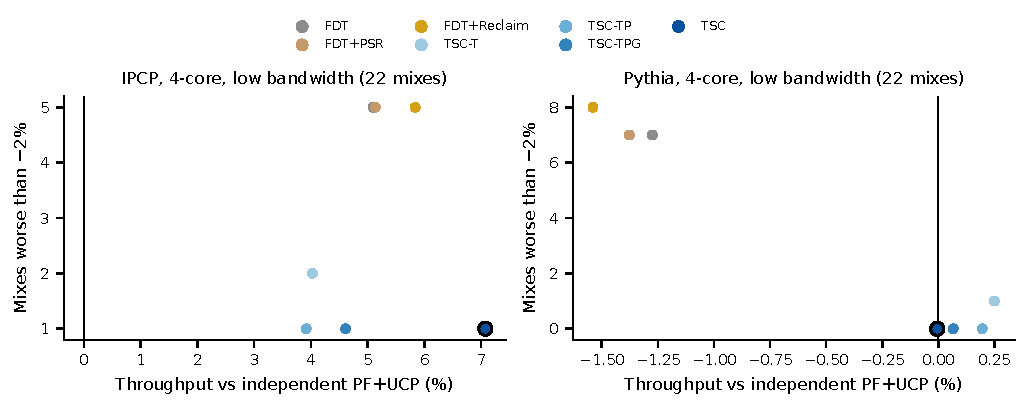
\includegraphics[width=0.9\textwidth]{tradeoff.pdf}
\caption{4-core, 2.4\,GB/s/core: throughput against the number of mixes that lose more than 2\%, for every design
(casualty counts: \cref{tab:final4}).  With IPCP, \vthree{} has the highest throughput and one mix below $-2\%$; with Pythia, all TSC variants are within
0.3\% of independent operation and the prior-style designs lose 1.3--1.5\%.}
\label{fig:tradeoff}
\end{figure*}

\Cref{tab:final4} and \cref{fig:tradeoff} summarise the 4-core results.

\paragraph{Low bandwidth, IPCP}
\vthree{} improves throughput by 7.1\% and harmonic speedup by 6.4\% over independent IPCP+UCP, the best of all
designs, with a single mix below $-2\%$ (worst $-2.9\%$).  The prior-style designs reach 5.1--5.8\% but have five mixes
below $-2\%$ and lose up to 16\%.  \vthree{} reduces the casualties from 30 to 25 and raises the mean worst core from
0.78 to 0.86 of its performance with neither mechanism; the prior-style designs reach 23--26 casualties and
0.91--0.93, with the mix losses above.  In the ablation, the throughput-safe acceptance (TSC-T) reduces the mixes
below $-2\%$ from 5 to 2 at 4.0\% throughput.  Adding the PSR-weighted partition (TSC-TP) changes throughput by
less than 0.2\% (4.0\% $\to$ 3.9\%); gradual re-enabling (TSC-TPG) raises it to 4.6\% and the accuracy hold
(\vthree) to 7.1\%.

\paragraph{Low bandwidth, Pythia}
Every prior-style design loses throughput (1.3--1.5\%, 7--8 mixes below $-2\%$).  \vthree{} causes no regression
(0.0\%, no mix below $-2\%$).  The static oracle finds only \OrcPyMean\% on average with Pythia.  It does not reduce Pythia's casualties (24 $\to$ 25), because these cores are victims of their neighbours'
\emph{useful} prefetching, which TSC largely keeps (see (iii) below).  Three observations from the 24 casualty cores of
the independent run (in 17 of the 22 mixes) support this.  (i)~They are cache-sensitive: 18 are HCLP (low prefetch sensitivity) and 5 HCHP, and their own median prefetch accuracy is only 0.37, against 0.82 over all
cores.  (ii)~Their neighbours prefetch well: the 72 co-running cores have a median accuracy of 0.83, and 60\% of them
run more than 2\% faster with both mechanisms than with neither (median speedup 1.12).  (iii)~Throttling those neighbours
does rescue them, at a net loss: FDT cuts the neighbours' issued prefetches to 37\%, the casualty cores speed up by
9.7\% on average, but the neighbours lose 6.0\% and the mixes 1.3\% of throughput.  TSC keeps 96\% of the
neighbours' prefetches, and both groups stay within 0.7\% of independent operation.  Rescuing the victims of useful
prefetching therefore costs throughput, i.e.\ the benefit of useful prefetchers, which our problem statement rules out.

\paragraph{Ample bandwidth}
At 9.6\,GB/s per core \vthree{} changes throughput by +0.6\% (IPCP) and $-0.2\%$ (Pythia), whereas the prior-style designs lose
0.8--1.9\% with up to eight mixes below $-2\%$ (worst $-16\%$).  Three IPCP mixes lose 2.0--2.4\% under \vthree{} (\cref{sec:limits}).

\begin{figure*}[!tp]
\centering
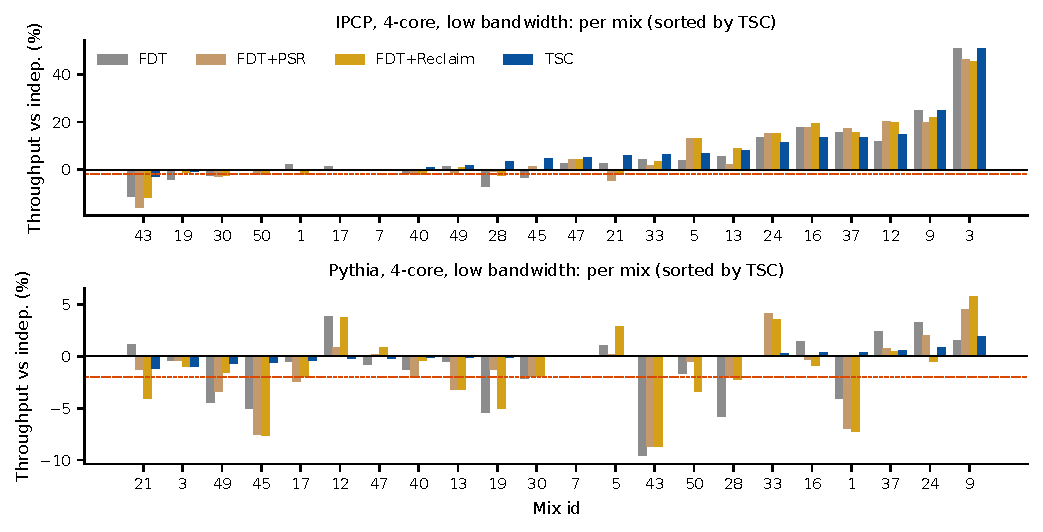
\includegraphics[width=0.9\textwidth]{permix_lowbw.pdf}
\caption{4-core, 2.4\,GB/s/core: per-mix throughput vs independent PF+UCP, sorted by \vthree.  Dashed line: $-2\%$.}
\label{fig:permix}
\end{figure*}

\begin{figure*}[!tp]
\centering
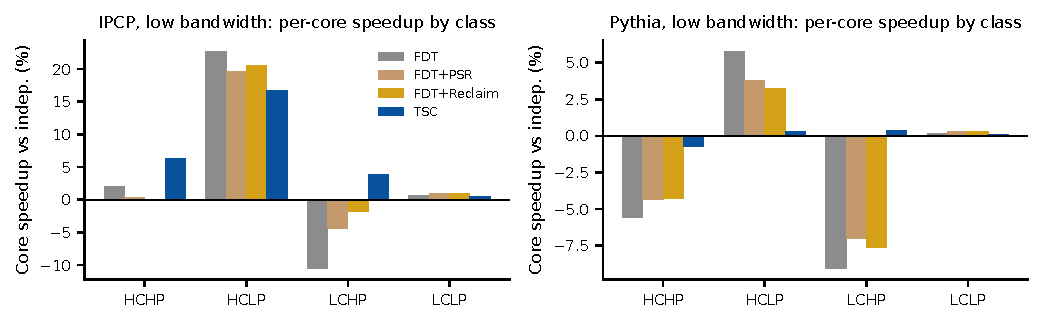
\includegraphics[width=0.9\textwidth]{byclass_lowbw.pdf}
\caption{4-core, 2.4\,GB/s/core: per-core speedup over independent PF+UCP by workload class.}
\label{fig:byclass}
\end{figure*}

\begin{figure*}[!tp]
\centering
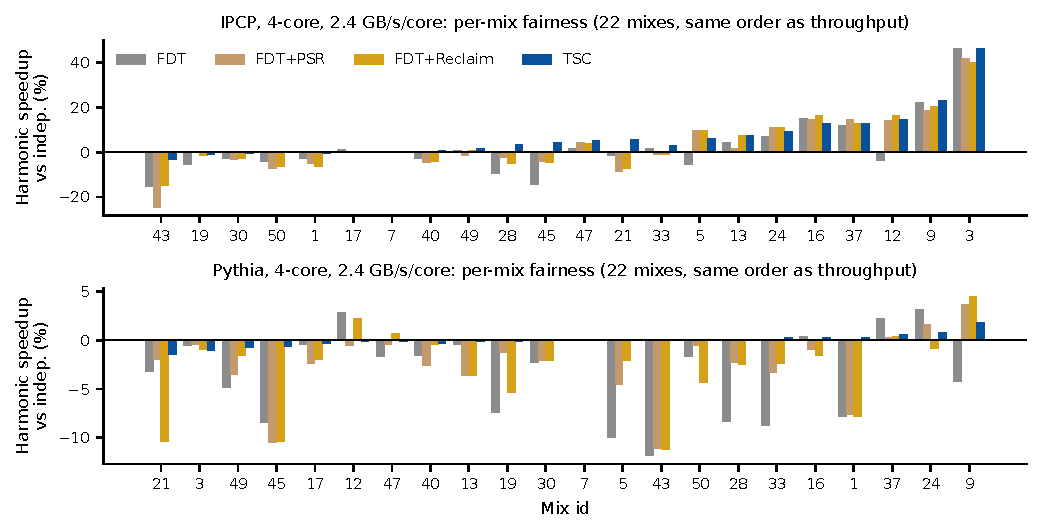
\includegraphics[width=0.9\textwidth]{hs_permix_lowbw.pdf}
\caption{4-core, 2.4\,GB/s/core: per-mix harmonic speedup (fairness) vs independent PF+UCP, mixes in the same order
as \cref{fig:permix}.}
\label{fig:hspermix}
\end{figure*}

\paragraph{Per mix and per class}
\Cref{fig:permix} shows the per-mix results: on the mixes where the prior-style designs gain most (right) \vthree{}
gains as well, and on the mixes where they lose (left) \vthree{} stays within 3\%.  By class (\cref{fig:byclass}), the cache-sensitive, prefetch-insensitive
cores (HCLP) gain the most with IPCP (+17\%); unlike FDT, \vthree{} does not sacrifice the LCHP cores,
whose prefetchers are useful ($-10\%$ under FDT, +4\% under \vthree).  \Cref{fig:hspermix} shows the same mixes for fairness: \vthree{} raises the harmonic speedup by more than 2\% in 13
of 22 IPCP mixes and lowers it by more than 2\% in one (worst $-3.0\%$), whereas the prior-style designs lower it by
more than 2\% in 8--10 IPCP and 11--12 Pythia mixes (worst $-24.8\%$).  With Pythia, \vthree{} stays within 2\% of
independent operation in every mix.

\subsection{8-core results}

\begin{table*}[!tp]
\centering
\caption{8-core, 2.4\,GB/s/core (columns as in \cref{tab:final4}).  All designs are compared on the mixes for which
\vthree{} has finished.}
\label{tab:eight}
\footnotesize
\begin{tabular}{llcccccc}
\toprule
& Design & Throughput & HS & Worst mix & Mixes $<-2\%$ & Casualties & Worst core \\
\midrule
\multicolumn{8}{l}{\emph{8-core, 2.4 GB/s/core, IPCP, 19 of 20 mixes (mix 05 pending)}} \\
& FDT & +7.4\% & +3.2\% & -7.9\% & 2 & 53$\to$49 & 0.70$\to$0.88 \\
& FDT+PSR & +3.6\% & +0.6\% & -13.8\% & 8 & 53$\to$57 & 0.70$\to$0.80 \\
& FDT+Reclaim & +4.3\% & +1.3\% & -7.6\% & 7 & 53$\to$55 & 0.70$\to$0.79 \\
& \textbf{TSC} & +6.0\% & +5.2\% & -1.2\% & 0 & 53$\to$48 & 0.70$\to$0.75 \\
\midrule
\multicolumn{8}{l}{\emph{8-core, 2.4 GB/s/core, Pythia, 19 of 20 mixes (mix 05 pending)}} \\
& FDT & -2.2\% & -5.4\% & -15.7\% & 8 & 37$\to$41 & 0.79$\to$0.89 \\
& FDT+PSR & -3.8\% & -5.8\% & -21.0\% & 9 & 37$\to$45 & 0.79$\to$0.82 \\
& FDT+Reclaim & -3.1\% & -4.8\% & -12.8\% & 12 & 37$\to$41 & 0.79$\to$0.83 \\
& \textbf{TSC} & +0.1\% & 0.0\% & -0.7\% & 0 & 37$\to$37 & 0.79$\to$0.79 \\
\bottomrule
\end{tabular}

\end{table*}

\Cref{tab:eight} compares the designs on the 19 of 20 8-core mixes for which \vthree{} has finished (mix 05 is still
running).

\paragraph{IPCP}
\vthree{} improves throughput by 6.0\% and harmonic speedup by 5.2\% with no mix below $-2\%$ (worst mix $-1.2\%$).
FDT reaches a higher throughput (7.4\%) but has two mixes below $-2\%$ (worst $-7.9\%$); FDT+PSR and FDT+Reclaim reach
3.6--4.3\% with 7--8 such mixes (worst $-13.8\%$).  \vthree{} has the highest harmonic speedup and the fewest
casualties (53 $\to$ 48, FDT 49), while FDT raises the mean worst core more (0.70 $\to$ 0.88, \vthree{} 0.75).

\paragraph{Pythia}
\vthree{} changes throughput by $+0.1\%$ with no mix below $-2\%$ (worst $-0.7\%$) and leaves the casualties
unchanged (37).  Every prior-style design loses throughput (2.2--3.8\%), has 8--12 mixes below $-2\%$ (worst
$-21.0\%$) and raises the casualties to 41--45.

\begin{figure*}[!tp]
\centering
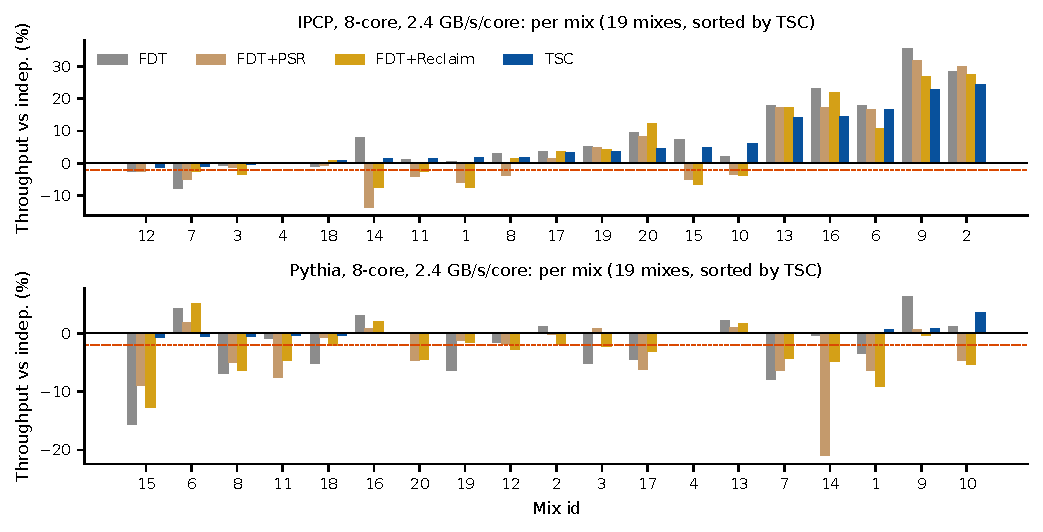
\includegraphics[width=0.9\textwidth]{permix_8core.pdf}
\caption{8-core, 2.4\,GB/s/core: per-mix throughput vs independent PF+UCP, sorted by \vthree{}, on the mixes for
which every design has finished.  Dashed line: $-2\%$.}
\label{fig:permix8}
\end{figure*}

\begin{figure*}[!tp]
\centering
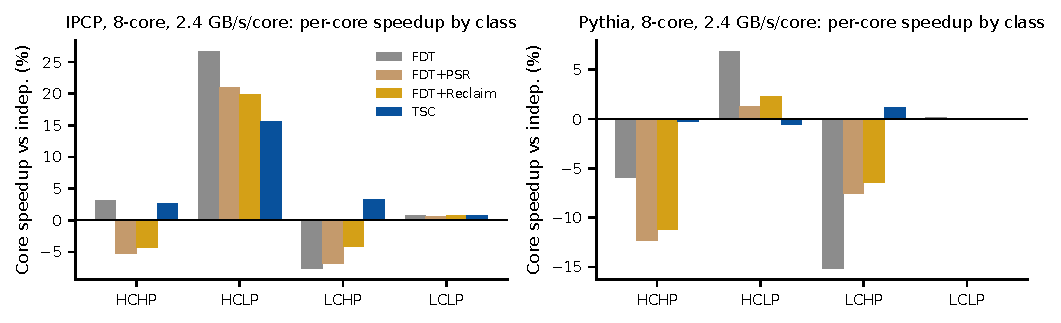
\includegraphics[width=0.9\textwidth]{byclass_8core_designs.pdf}
\caption{8-core, 2.4\,GB/s/core: per-core speedup over independent PF+UCP by workload class, on the same mixes as
\cref{fig:permix8}.}
\label{fig:byclass8}
\end{figure*}

\begin{figure*}[!tp]
\centering
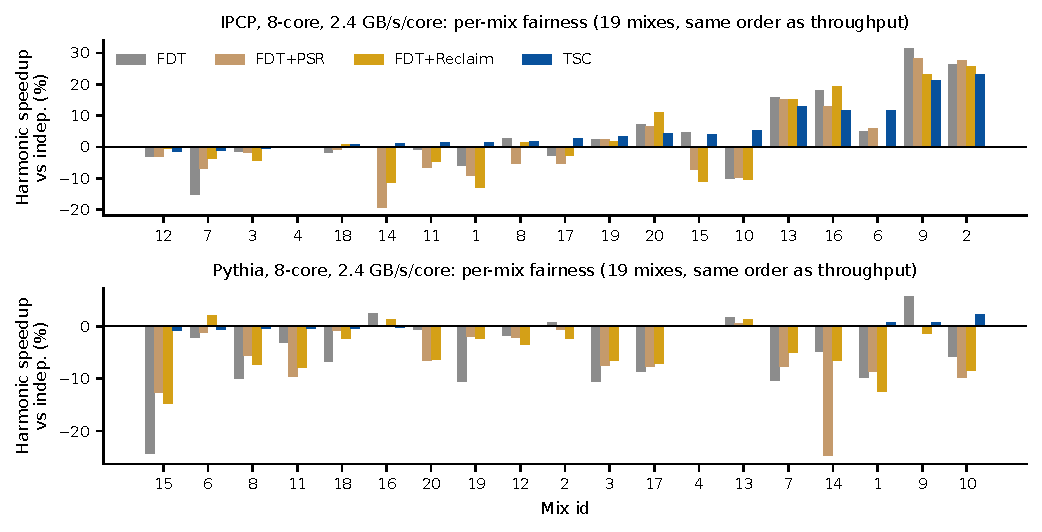
\includegraphics[width=0.9\textwidth]{hs_permix_8core.pdf}
\caption{8-core, 2.4\,GB/s/core: per-mix harmonic speedup (fairness) vs independent PF+UCP, mixes in the same order as
\cref{fig:permix8}.}
\label{fig:hspermix8}
\end{figure*}

\Cref{fig:permix8,fig:hspermix8,fig:byclass8} show the 8-core results per mix (throughput and fairness) and per
workload class.

\subsection{Sensitivity}
\label{sec:sweep}

\begin{table}[!htbp]
\centering
\caption{Sensitivity of \vthree{}, 4-core, 2.4\,GB/s/core: throughput change relative to \vthree{} with default
parameters on the same mixes, one parameter changed at a time.}
\label{tab:sweep}
\footnotesize
\begin{tabular}{lcrcc}
\toprule
Parameter (default) & Value & Mixes & IPCP & Pythia \\
\midrule
Accuracy hold (0.15) & 0.10 & 10 & -1.3\% & -0.2\% \\
Accuracy hold (0.15) & 0.20 & 10 & +0.5\% & -0.1\% \\
Own-core budget (1\%) & 3\% & 22 & -0.1\% & +0.0\% \\
\bottomrule
\end{tabular}

\end{table}

\Cref{tab:sweep} varies the parameters that only \vthree{} has, one at a time.  Raising the accuracy hold from 0.15 to 0.20 changes IPCP throughput by $+0.5\%$, lowering it to 0.10 by
$-1.3\%$; Pythia changes by at most 0.2\%.  Relaxing the own-core budget from 1\% to 3\% changes throughput by at
most 0.1\%.  The
mechanisms that \vthree{} shares with the prior-style designs (two-level drop, victim guard, partition step) were
swept on FDT+Reclaim during the design; there, only disabling the two-level drop, a 5\% victim guard and a one-way
partition step cost more than 1\%, so we kept their reference values.

\subsection{Limitations}
\label{sec:limits}
\begin{itemize}
  \item \textbf{Ample bandwidth.}  In the three IPCP mixes that lose 2.0--2.4\% at 9.6\,GB/s per core, single cores
        lose 4.5--8.4\%.  In mix 49 a core with accuracy 0.05 is held at level 1 for 441 of 466 epochs and loses
        8.4\%, although with both mechanisms it runs 6.5\% faster than with neither; in mix 12 a core with accuracy
        0.07 loses 6.6\%; in mix 1 two cores with accuracy 0.19 and 0.32 are throttled in 17--18\% of the epochs and
        lose 4.5\% and 6.3\%.  Letting a calm DRAM release held cores as well is one option we have not evaluated.
  \item \textbf{Static headroom at ample bandwidth.}  At 9.6\,GB/s per core the static oracle finds \OrcIpMean\% for
        IPCP (on its \OrcIpN{} mixes), whereas \vthree{} gains 0.6\% (on 22 mixes).  \vthree{} throttles only when
        DRAM is busy; whether an own-core test that runs also when DRAM is calm captures this headroom is open.
  \item \textbf{Victims of useful prefetching} are not rescued (Pythia, \cref{sec:experiments}).
  \item \textbf{Measurement noise}: decisions rest on two-epoch IPC measurements.
  \item \textbf{Context switches} do not occur in our trace-driven runs; on a real system a core's level and
        statistics would be reset on a context switch.
\end{itemize}

\section{Conclusion and Future Work}
\label{sec:conclusion}

On 8 cores at 2.4\,GB/s per core, independent prefetching and UCP leave 36\% (IPCP) and 26\% (Pythia) of the cores
more than 2\% slower than with neither mechanism, UCP gives extra ways to cores with inaccurate IPCP prefetchers, and
a static oracle finds up to 38\% of headroom.  Feedback throttling that keeps a step when fairness improves keeps the
cores that prefetching speeds up by at least 1.3$\times$ throttled about 90\% of the time and loses up to 16\% on
individual mixes.

We presented TSC, a modular coordinator that keeps a throttle step only if the IPC measured after it shows at most 0.5\%
throughput loss and at most 1\% loss for the throttled core, re-tests every throttle, holds prefetchers with an
accuracy below 0.15 down, and weights the partitioner's utility by each core's prefetch success rate.  It needs no
change to IPCP or Pythia and about 84 bytes of state per core.  On 22 4-core mixes at 2.4\,GB/s per core it
improves throughput by 7.1\% over independent IPCP+UCP with one mix below $-2\%$, against five such mixes and losses
of up to 16\% for prior-style designs, changes Pythia's throughput by 0.0\% where every prior-style design loses 1.3--1.5\%, and changes throughput by
$+0.6\%$ (IPCP) and $-0.2\%$ (Pythia) at 9.6\,GB/s per core.
On 8 cores at 2.4\,GB/s per core (19 of 20 mixes) it improves throughput by 6.0\% (IPCP) and 0.1\% (Pythia) with no
mix below $-2\%$; FDT gains more with IPCP (7.4\%) but has two such mixes, and every prior-style design loses
2.2--3.8\% with Pythia.

\paragraph{Future work}
\begin{itemize}
  \item Confine the accuracy hold to periods of DRAM pressure, and test prefetchers for self-harm also when DRAM is
        calm, to reach the static headroom at ample bandwidth (\cref{sec:limits}).
  \item Replace the hand-set acceptance thresholds with a learned policy, using the keep-or-revert trials as its
        reward signal.  Online reinforcement learning already controls a single prefetcher
        (Pythia~\cite{bera2021pythia}), the aggressiveness of the prefetchers of several cores
        (APAC~\cite{yang2025apac}) and the joint use of several prefetchers and an off-chip predictor
        (Athena~\cite{bera2026athena}); extending such an agent to the LLC partition is the natural next step.
  \item Rescue victims of useful prefetching with DRAM bandwidth partitioning~\cite{holtryd2021cbp} rather than by
        throttling, which the throughput budget forbids.
  \item Lower-noise measurement, e.g.\ set dueling for the partition and longer, interleaved trials.
  \item More prefetchers (SPP, Bingo, Berti) and core counts beyond 8.
\end{itemize}


\IfFileExists{IEEEtran.bst}{\bibliographystyle{IEEEtran}}{\bibliographystyle{plain}}
\bibliography{refs}

\appendix
\section{Static Oracle: All Evaluated Configurations}
\label{app:oracle}

\Cref{fig:scatterpy,fig:scatter8} complete \cref{fig:scatter}: every fixed configuration the per-core oracle evaluated
for UCP+Pythia on 4 cores and for UCP+IPCP on 8 cores at 2.4\,GB/s per core.  \Cref{tab:oracle4mix,tab:oracle8mix}
list the per-mix results.

\begin{figure*}[!htbp]
\centering
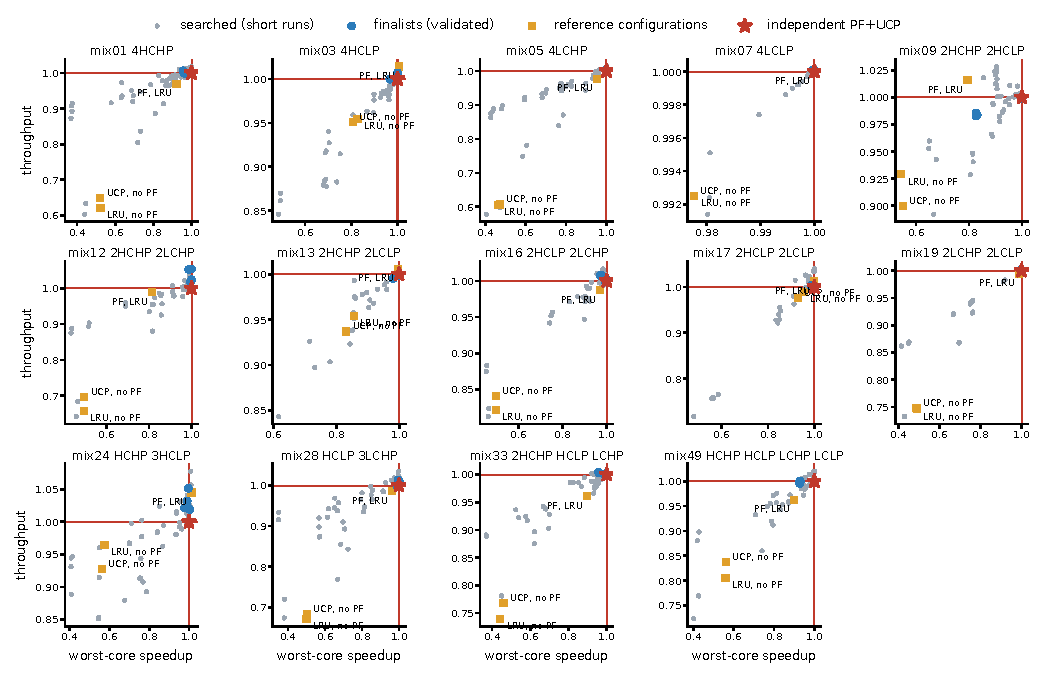
\includegraphics[width=0.9\textwidth]{oracle_scatter_pythia.pdf}
\caption{Per-core static oracle, 4-core, 9.6\,GB/s/core, UCP+Pythia (axes and marks as in \cref{fig:scatter}).}
\label{fig:scatterpy}
\end{figure*}

\begin{figure*}[!htbp]
\centering
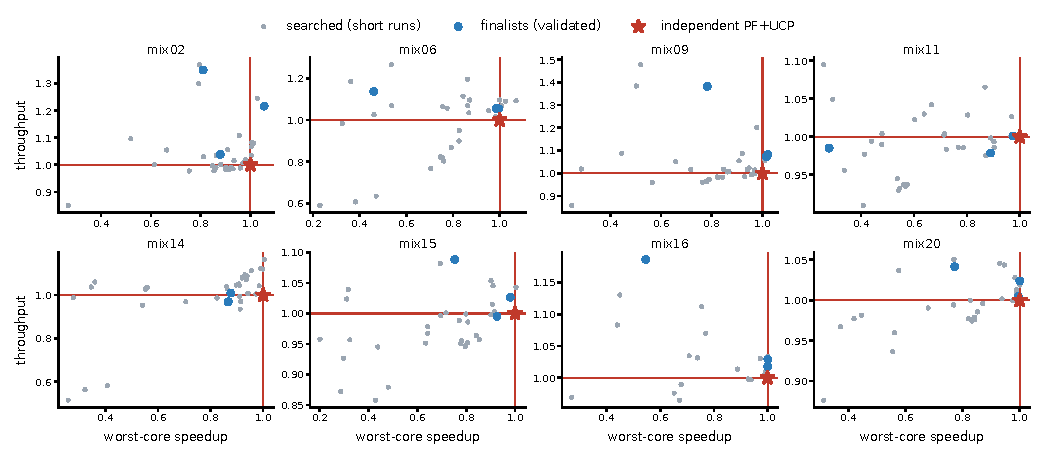
\includegraphics[width=0.95\textwidth]{oracle_scatter_8core.pdf}
\caption{Per-core static oracle, 8-core UCP+IPCP at 2.4\,GB/s/core, axes as in \cref{fig:scatter}.  Many
configurations gain throughput, but the largest gains mostly lie to the left of the star: they sacrifice a core.}
\label{fig:scatter8}
\end{figure*}

\begin{table*}[!htbp]
\centering
\caption{Per-core static oracle, 4-core, 9.6\,GB/s/core: per mix, the best throughput found at the search length when
searching only the prefetch knob, only the partition or both, and the best and the fairest configuration that does not
lose throughput after validation at full length.  Throughput (Thr.) and worst core are relative to independent
operation.  Configuration: ``UCP'' = UCP's adaptive ways, ``ways a/b/c/d'' = fixed ways per core; c$k$ = core $k$,
``cap $d$'' = degree cap $d$, ``off'' = prefetcher off, unlisted cores native.}
\label{tab:oracle4mix}
\footnotesize
\resizebox{\textwidth}{!}{\begin{tabular}{llccclcclcc}
\toprule
 & & \multicolumn{3}{c}{Search length: best of} & \multicolumn{3}{c}{Best validated (throughput)} & \multicolumn{3}{c}{Fairest validated, no throughput loss} \\
\cmidrule(lr){3-5}\cmidrule(lr){6-8}\cmidrule(lr){9-11}
PF & Mix & PF knob & Partition & Both & Configuration & Thr. & Worst & Configuration & Thr. & Worst \\
\midrule
IPCP & 1 & 1.002 & 1.016 & 1.012 & ways 6/1/2/7 & 0.999 & 0.989 & ways 6/1/2/7; c0 cap 4 & 0.999 & 0.991 \\
IPCP & 3 & 1.159 & 1.001 & 1.111 & UCP; all off & 1.172 & 1.074 & UCP; all cap 1 & 1.165 & 1.079 \\
IPCP & 5 & 1.041 & 1.022 & 1.054 & UCP; c1 cap 1 & 1.028 & 1.012 & ways 1/6/1/8; c1 cap 1 & 1.026 & 1.013 \\
IPCP & 7 & 1.000 & 1.000 & 0.999 & UCP; c1 cap 2 & 1.000 & 1.000 & ways 1/5/7/3 & 1.000 & 1.000 \\
IPCP & 9 & 1.119 & 1.042 & 1.019 & UCP; c0 off & 1.108 & 1.010 & UCP; c0 off & 1.108 & 1.010 \\
IPCP & 12 & 1.036 & 1.002 & 1.054 & ways 1/1/1/13; c3 cap 1 & 1.072 & 1.012 & ways 3/1/1/11; c3 cap 1 & 1.051 & 1.013 \\
IPCP & 13 & 1.030 & 0.952 & 1.012 & UCP; c0 cap 1, c2 cap 1 & 1.028 & 1.002 & UCP; c2 off & 1.024 & 1.002 \\
IPCP & 16 & 1.055 & 1.018 & 1.047 & UCP; c0 cap 1, c2 cap 1 & 1.049 & 1.008 & UCP; c0 cap 1, c2 off & 1.049 & 1.010 \\
IPCP & 17 & 1.006 & 1.042 & 1.047 & ways 4/1/1/10; c3 cap 2 & 1.006 & 0.998 & ways 4/1/1/10; c3 cap 2 & 1.006 & 0.998 \\
IPCP & 19 & 1.016 & 1.008 & 1.019 & ways 4/4/4/4; c1 cap 4, c2 cap 4, c3 cap 4 & 1.007 & 0.994 & ways 6/5/1/4 & 1.002 & 1.000 \\
IPCP & 24 & 1.079 & 1.022 & 0.932 & UCP; c0 off & 1.087 & 1.003 & UCP; c0 off & 1.087 & 1.003 \\
IPCP & 28 & 1.078 & 1.067 & 1.100 & ways 1/1/5/9; c3 off & 1.057 & 1.013 & ways 1/1/5/9; c3 off & 1.057 & 1.013 \\
IPCP & 33 & 1.017 & 1.008 & 0.969 & UCP; all cap 4 & 1.036 & 0.962 & UCP; c3 cap 2 & 1.010 & 1.000 \\
IPCP & 49 & 1.003 & 1.024 & 1.025 & ways 1/1/1/13; c1 cap 2 & 0.991 & 0.890 & ways 1/1/1/13; c1 cap 2 & 0.991 & 0.890 \\
\midrule
Pythia & 1 & 0.993 & 1.018 & 1.014 & ways 2/1/1/12 & 1.006 & 0.956 & ways 2/1/1/12; c1 cap 4 & 1.003 & 0.957 \\
Pythia & 3 & 0.994 & 1.000 & 0.886 & UCP; c1 off & 1.007 & 1.000 & UCP; c1 off & 1.007 & 1.000 \\
Pythia & 5 & 1.001 & 1.013 & 1.012 & ways 1/7/1/7 & 1.004 & 0.997 & ways 1/7/1/7; c1 cap 1 & 1.000 & 1.000 \\
Pythia & 7 & 1.000 & 1.000 & 0.999 & ways 1/3/11/1 & 1.000 & 1.000 & ways 1/7/7/1 & 1.000 & 1.000 \\
Pythia & 9 & 1.018 & 1.024 & 1.028 & UCP; c1 cap 2 & 1.001 & 1.000 & UCP; c1 cap 2 & 1.001 & 1.000 \\
Pythia & 12 & 1.017 & 1.018 & 1.032 & ways 1/2/1/12; c1 cap 4 & 1.054 & 0.999 & ways 1/2/1/12 & 1.023 & 1.000 \\
Pythia & 13 & 1.000 & 0.993 & 0.938 & UCP; c0 cap 4 & 1.000 & 0.999 & UCP; c0 cap 4 & 1.000 & 0.999 \\
Pythia & 16 & 1.003 & 1.015 & 1.016 & ways 6/8/1/1; c2 cap 2 & 1.008 & 0.971 & UCP; c2 cap 4 & 1.001 & 1.000 \\
Pythia & 17 & 1.002 & 1.039 & 1.040 & ways 3/1/1/11; c1 cap 4 & 1.004 & 0.987 & ways 3/1/1/11; c1 cap 4 & 1.004 & 0.987 \\
Pythia & 19 & 1.001 & 1.003 & 1.003 & ways 7/5/1/3; c2 cap 4 & 1.002 & 0.997 & ways 7/5/1/3 & 1.000 & 1.000 \\
Pythia & 24 & 1.025 & 1.042 & 1.078 & ways 6/8/1/1; c0 off & 1.052 & 0.996 & UCP; c0 off & 1.019 & 1.004 \\
Pythia & 28 & 1.011 & 1.025 & 1.035 & ways 3/1/1/11; c3 off & 1.014 & 0.996 & UCP; c3 off & 1.011 & 1.001 \\
Pythia & 33 & 1.002 & 1.002 & 1.006 & ways 12/1/1/2; c3 cap 2 & 1.004 & 0.956 & UCP; c0 cap 4 & 1.001 & 0.993 \\
Pythia & 49 & 1.003 & 1.020 & 1.020 & ways 1/1/1/13 & 1.000 & 0.930 & ways 1/1/1/13 & 1.000 & 0.930 \\
\bottomrule
\end{tabular}
}
\end{table*}

\begin{table*}[!htbp]
\centering
\caption{Per-core static oracle, 8-core UCP+IPCP, 2.4\,GB/s/core: per mix, the best and the fairest configuration
that does not lose throughput after validation (notation as in \cref{tab:oracle4mix}), and the search summary.}
\label{tab:oracle8mix}
\footnotesize
\begin{tabular}{rlccclcc}
\toprule
 & \multicolumn{4}{c}{Best validated (throughput)} & \multicolumn{3}{c}{Fairest validated, no throughput loss} \\
\cmidrule(lr){2-5}\cmidrule(lr){6-8}
Mix & Configuration & Knob & Thr. & Worst & Configuration & Thr. & Worst \\
\midrule
2 & UCP; all off & prefetch only & 1.350 & 0.810 & UCP; all cap 2 & 1.216 & 1.055 \\
6 & UCP; all off & prefetch only & 1.137 & 0.461 & UCP; c1 off & 1.053 & 0.996 \\
9 & UCP; all off & prefetch only & 1.382 & 0.783 & UCP; c1 off & 1.082 & 1.021 \\
11 & UCP; c4 cap 2 & prefetch only & 1.001 & 0.975 & UCP; c4 cap 2 & 1.001 & 0.975 \\
14 & ways 1/1/4/6/1/1/1/1 & partition only & 1.009 & 0.877 & ways 1/1/4/6/1/1/1/1 & 1.009 & 0.877 \\
15 & UCP; c2 off & prefetch only & 1.089 & 0.753 & UCP; c6 off & 1.027 & 0.980 \\
16 & UCP; all off & prefetch only & 1.186 & 0.546 & UCP; c1 off & 1.029 & 1.001 \\
20 & UCP; all cap 2 & prefetch only & 1.041 & 0.772 & UCP; c7 cap 2 & 1.024 & 1.000 \\
\midrule
\multicolumn{8}{l}{Search length, mean of the best per mix: prefetch knob only 1.198, partition only 1.044, both knobs 0.976} \\
\multicolumn{8}{l}{Configurations evaluated in total over the 8 mixes: prefetch only 144, partition only 88, both knobs 16} \\
\bottomrule
\end{tabular}

\end{table*}
   % appendix after the references

\end{document}
